\documentclass{report}
\usepackage{graphicx}
\usepackage[dvipsnames]{xcolor}
\usepackage[most]{tcolorbox}
\usepackage{amsmath}
\usepackage{pgfplots}
\usepgfplotslibrary{fillbetween}
\pgfplotsset{width=10cm,compat=1.9}

\usepackage[letterpaper,top=2cm,bottom=2cm,left=2cm,right=2cm,marginparwidth=1.75cm]{geometry}
\setlength\parindent{15pt}

\usepackage[unicode]{hyperref}
\hypersetup{colorlinks,
  allcolors=[RGB]{010 090 200}}

\usepackage[T2A]{fontenc}
\usepackage[russian]{babel}
\usepackage{indentfirst}

\newcommand{\mycolor}[1]{RoyalBlue!#1!white}
\newcommand{\mycolorframe}{100}
\newcommand{\mycolorlower}{100}
\newcommand{\mycolorupper}{100}
\newcommand{\mycolorback}{10}
\newcommand{\mycolortext}{black}

\newtcolorbox{mybox}[1]{breakable,colupper=\mycolortext,colframe=\mycolor{\mycolorframe},colback=\mycolor{\mycolorback},collower=\mycolortext,fonttitle=\bfseries,title={#1}}
\newtcolorbox{mybox_2}{breakable,colupper=\mycolortext,colframe=\mycolor{\mycolorframe},colback=\mycolor{\mycolorback},collower=\mycolortext,fonttitle=\bfseries}

%\let\oldtableofcontents\tableofcontents
%\renewcommand{\tableofcontents}{
%\begin{tcolorbox}[breakable,colback=\mycolor{\mycolorback},colframe=\mycolor{\mycolorframe},collower=\mycolor{\mycolorlower},colupper=\mycolor{\mycolorupper}]
%    \oldtableofcontents
%\end{tcolorbox}}




\begin{document}

\newgeometry{left=4.5cm,right=4.5cm}
\thispagestyle{plain}
\begin{titlepage}
    \hfill\begin{center}
        \begin{tcolorbox}[
            collower=\mycolor{\mycolorlower},
            colupper=\mycolor{\mycolorupper},
            colframe=\mycolor{\mycolorframe},
            colback=\mycolor{\mycolorback},
            fonttitle=\Large\bfseries\centering,
            title=Модель Хотеллинга. Сигналинг. Вертикальная дифференциация товара
        ]
        \large\centering\textbf{Хендбук по олимпиадной экономике}
        \tcblower
        \centering\textbf{Тумаков Николай}
        \end{tcolorbox}
    \end{center}
\end{titlepage}

\restoregeometry

\tableofcontents



\chapter{Введение}


\section{Первые шаги}
\indent\setlength{\parindent}{1em}Перед началом прохождения пособия я настоятельно Вам вступить в наше
\textbf{\href{https://t.me/econ_handbook_screening}{телеграм-сообщество}}. Там Вы найдете всю актуальную информацию и
сможете узнать ответы на все свои вопросы.\\
\indent\setlength{\parindent}{1em}Буду очень Вам благодарен, если вы заполните \textbf{\href{https://forms.gle/bW7CD2zcdUhnbFnR7}{форму регистрации}}. Так вы поддерживаете
этот проект, как индивидуальную выпускную работу.\\
\indent\setlength{\parindent}{1em}Но главное в этих действиях для Вас это создание некоторого коммитнмент для прохождения этого хендбука. То есть Вы создаете дополнительную мотивацию именно для себя! Желаю Вам удачи!

\section{Для кого}
\indent\setlength{\parindent}{1em}Если ты освоил основные темы олимпиадной экономики, хочешь расширить свой кругозор и готов активно учиться и решать задачи, то этот хендбук точно для тебя.

\section{Взаимодействие с хендбуком и структура}
\indent\setlength{\parindent}{1em}Хендбук разделен на большие темы и подтемы. Структура каждого блока включает в себя блоки:
\begin{enumerate}
    \item Вся необходимая теория
    \item Графическая иллюстрация для лучшего понимания
    \item Разбор модели в общем виде
    \item Примеры задач с решением
    \item Подборка из различных задач
    \item Подборка задач из олимпиад
    \item Тест в гугл форме для проверки ответов на задачи
\end{enumerate}

\section{Советы по работе с хендбуком}
\begin{enumerate}
    \item Пробуйте решить задач с решением. Если Вы сами догадаетесь до решения это будет в разы полезнее.
    \item Повторяйте пройденное время от времени
\end{enumerate}

\section{Об авторе}
\indent\setlength{\parindent}{1em}Меня зовут Тумаков Николай. Я учусь в Лицее НИУ ВШЭ на направлении МатЭк выпуска 2024 года. Мой опыт участия в олимпиадах начался с 9 класса. В 9 классе у меня получилось пройти на Заключительный Этап ВСОШ. В 10 классе я взял диплом победителя МОШ за 11 класс. Учился на многих онлайн курсах и выездных школах. \\
\indent\setlength{\parindent}{1em}Готов представить Вам мой хендбук, желаю насладиться решение составленного мной хендбука!

\section{Контакты}
\indent\setlength{\parindent}{1em}При обнаружении опечаток или ошибок в хендбуке, тестах, подборках Вы можете написать мне в личные сообщения в \textbf{\href{https://t.me/nntumakov}{телеграм}}.\\
\indent\setlength{\parindent}{1em}Также у хендбука есть свое \textbf{\href{https://t.me/econ_handbook_screening}{телеграм-сообщество}}. Там можно задать вопрос в соответствующем топике. Но если вы хотите написать мне лично, то используйте личные сообщения \textbf{\href{https://t.me/nntumakov}{телеграм}}, где я Вам также смогу ответить.

\section{Помогите автору сдать ИВР}
\indent\setlength{\parindent}{1em}Данный хендбук является моей индивидуальной выпускной работой. Я хочу привнести в мир олимпиадной подготовки новый материал, который поможет ознакомится с необычными темами олимпиадной экономики.\\
\indent\setlength{\parindent}{1em}Вы можете мне помочь, заполняя гугл-формы на протяжении прохождения хендбука. Особенно важно заполнить форму с регистрацией, где вы отметитесь, что решили пройти этот материал. Также если вам захочется можно заполнить форму с фидбеком. Также я буду Вам благодарен, если вы будете дальше распространять этот материал.\\
\begin{center}
    \textbf{\textit{\href{https://forms.gle/bW7CD2zcdUhnbFnR7}{Гугл-форма для регистрации}}}\\\\
    \textbf{\textit{\href{https://forms.gle/31gene8PMRuqCLvr9}{Гугл-форма для фидбека}}}
\end{center}

\section{Благодарности и информация о научном консультанте}
\indent\setlength{\parindent}{1em}Хочу поблагодарить за помощь прямую и косвенную в подготовке этого хендбука:
\begin{enumerate}
    \item \textbf{А.Н.Челеховский} - мой учитель экономики и научный консультант у этого хендбука
    \item \textbf{Лука Логинов} - преподаватель олмат.экономика, где я впервые услышал лекцию по теме Сигналинг
    \item \textbf{Александр Шиваров} - руководитель олмат.экономика, где я услышал лекцию по теме Вертикальная дифференциация товара
\end{enumerate}



\chapter{Вспомогательные темы}


\section{Равновесие в теории игр}

\indent\setlength{\parindent}{1em}Приведу базовые понятия теории игр. Они могут пригодится в третьей главе 4.

\begin{mybox}{Равновесие по Нэшу}
    Ситуация, при котором ни один игрок не может улучшить свое положение, изменяя свою стратегию, при условии, что
    остальные игроки сохраняют свои стратегии неизменными.
\end{mybox}

\begin{mybox}{Эффективность по Парето}
    Ситуация, когда нельзя улучшить положение ни одного из игроков, не ухудшая при этом положения другого.
\end{mybox}

Эти понятия описывают различные ситуации. Не обязательно равновесие по Нэшу является эффективном по Парето.
\smallskip\\\indent\setlength{\parindent}{1em} \textbf{Например:} В модели Курно игроки при неизменных стратегиях
других агентов не могут улучшить своего положения. Тем не менее эффективное по Парето равновесие является иным. Например
с точки зрения производителей, эффективным по Парето будет производство монопольного выпуска. А с точки зрения
общественного благосостояния - равновесие при совершенной конкуренции (при условии отсутствия отрицательных внешних
эффектов)\smallskip\\\indent\setlength{\parindent}{1em} Для дальнейшего понимания материала будет полезно
классифицировать типы равновесия. Возможно в других темах данные понятия можно будет определить по-другому. Определим
что это будет значить конкретно в наших темах

\newpage


\section{Скрининг}

\subsection{Теория}

\indent\setlength{\parindent}{1em} Согласно А. Пигу ценовую дискриминацию делят на три категории. Скрининг относится
ко второму типу дискриминации.

\begin{mybox}{Скрининг}
    Процесс разделение потребителей на группы с помощью их собственнного самоопределения в результате максимизации
    полезности. В этой модели производитель не умеет различать группы производителей, но знает их предпочтения.
    Производитель решает с конца и назначает соответствующие контракты группам.
\end{mybox}


\subsection{Практика}

Теперь разберем, как решать задачи на скрининг на примере.

\begin{mybox}{Самая базовая задача}
    \textbf{Условие:}\\ Монополист может предлагать любые комплекты $(x_1;P_1)$. Существует 2 группы, одинаковые по
    численности, каждый потребитель из каждой покупает по одному комплекту. Они выбирают какой комплект купить исходя из
    максимизации своих функций полезности. \\
    $$U_1(x_1,C_1)=40x_1-x_1^2-C_1$$
    $$U_2(x_2,C_2)=32x_2-x_2^2-C_2$$
    $$TC=4X\text{,}\;X=x_1+x_2$$
    \tcblower
    \textbf{Решение:}
    \begin{enumerate}
        \item Набор комплектов будет единственным, иначе нам не будет смысла предлагать третий не самый выгодный
        комплект
        \item Не теряя общности, можем предполагать, что существует по одному потребителю каждого типа, так как издержки
        монополиста обладают постоянной отдачей из масштаба.
        \item Возможны два равновесия. \begin{enumerate}
            \item Продаем различные комплекты разным группам (включает в себя случай когда продаем одинаковые комплекты
            разным группам)
            \item Продаем только платежеспособной группе, так как не хотим сильно занижать цену дорогого комлекта.
        \end{enumerate}
        \item Для начала рассмотрим ситуацию, когда мы продаем обоим группам.
        \item Наша задача выбрать оптимальные $(P_1;x_1);(P_2;x_2)$. Прибыль в общем виде выглядит:
        $$\Pi=P_1+P_2-TC(x_1+x_2)=P_1+P_2-4(x_1+x_2)$$
        \item Запишем необходимые и достаточные условия, а затем я разберу, что они значат.
        \begin{equation*}
         \begin{cases}
           (1)\;U_1(x_1,P_1)\geq U_1(x_2,P_2)
           \\
           (2)\;U_1(x_1,P_1)\geq 0
           \\
           (3)\;U_2(x_2,P_2)\geq U_2(x_1,P_1)
           \\
           (4)\;U_2(x_2,P_2)\geq 0
         \end{cases}
        \end{equation*}
        (1) Комплект-1 лучше чем комплект-2 для 1 агента (то есть тот, который для него предназначается)\\
        (2) Лучше купить комплект-1, чем ничего не покупать\\
        (3) Комплект-2 лучше чем комплект-1 для 2 агента (то есть тот, который для него предназначается)\\
        (4) Лучше купить комплект-2, чем ничего не покупать
        \item Подставим наши циферки
        \begin{equation*}
         \begin{cases}
           (1)\;40x_1-x_1^2-P_1\geq 40x_2-x_2^2-P_2
           \\
           (2)\;40x_1-x_1^2-P_1\geq 0
           \\
           (3)\;32x_2-x_2^2-P_2\geq 32x_1-x_1^2-P_1
           \\
           (4)\;32x_2-x_2^2-P_2\geq 0
         \end{cases}
        \end{equation*}
        \item Заметим, что из (1) и (4) следует (2):
        $$40x_1-x_1^2-P_1\geq 40x_2-x_2^2-P_2\geq 32x_2-x_2^2-P_2\geq 0$$
        Таким образом можем убрать (2) из системы:
        \begin{equation*}
         \begin{cases}
           (1)\;40x_1-x_1^2-P_1\geq 40x_2-x_2^2-P_2
           \\
           (3)\;32x_2-x_2^2-P_2\geq 32x_1-x_1^2-P_1
           \\
           (4)\;32x_2-x_2^2-P_2\geq 0
         \end{cases}
        \end{equation*}
        \item При фиксированных $x_1;x_2$ увеличение цены строго увеличит $\Pi$. Таким образом, можем повышать $P_1$, до тех пор, пока (1) уравнение не сойдется в равенство. Это не нарушает уравнение (3), так как это ухудшает комплект-1 для 2-го агента, а значит правая часть уменьшается и знак не изменится.
        \begin{equation*}
         \begin{cases}
           (1)\;40x_1-x_1^2-P_1= 40x_2-x_2^2-P_2
           \\
           (3)\;32x_2-x_2^2-P_2\geq 32x_1-x_1^2-P_1
           \\
           (4)\;32x_2-x_2^2-P_2\geq 0
         \end{cases}
        \end{equation*}
        \item Также хочется повысить цену $P_2$. Заметим, если мы будет повышать $P_1$ и $P_2$ на одинаковую величину, то в уравнениях (1) и (2) знак не может поменятся, а (4) сойдется в равенство
        \begin{equation*}
         \begin{cases}
           (1)\;40x_1-x_1^2-P_1= 40x_2-x_2^2-P_2
           \\
           (3)\;32x_2-x_2^2-P_2\geq 32x_1-x_1^2-P_1
           \\
           (4)\;32x_2-x_2^2-P_2= 0
         \end{cases}
        \end{equation*}
        \item Вычтем из (1) уравнение (3), получим:
        \begin{equation*}
         \begin{cases}
           (1)\;40x_1-x_1^2-P_1= 40x_2-x_2^2-P_2
           \\
           (3)\;x_1\geq x_2
           \\
           (4)\;32x_2-x_2^2-P_2= 0
         \end{cases}
        \end{equation*}
        \item Выразим $P_1(x_1;x_2)$ и $P_2(x_1;x_2)$:
        $$P_2=32x_2-x_2^2$$
        $$P_1=40x_1-x_1^2-40x_2+x_2^2+P_2=40x_1-x_1^2-8x_2$$
        \item Подставив $P_1(x_1;x_2);P_2(x_1;x_2)$ в $\Pi$ получаем зависимость $\Pi(x_1;x_2)$, максимизируем по двум переменным:
        $$\Pi(x_1;x_2)=P_1(x_1;x_2)+P_2(x_1;x_2)-TC(x_1+x_2)=32x_2-x_2^2+40x_1-x_1^2-8x_2-4x_1-4x_2=$$
        $$\Pi(x_1;x_2)=20x_2-x_2^2+36x_1-x_1^2\xrightarrow{x_1;x_2} \max$$
        \item Получили 2 независимые параболы ветвями вниз, максимум в вершине: $(x_1;P_1)=(18;316)$, $(x_2;P_2)=(10;220)$, $\Pi=424$. Ограничение $x_1\geq x_2$ - истинно
        \item Осталось рассмотреть случай, когда мы продаем только платежеспособному агенту. То есть назначаем один комплект. Нам имеет смысл занулить его излишек. Таким образом $P_1=40x_1-x_1^2$
        \item Записываем целевую функцию: $$\Pi(x_1)=P_1-4x_1=36x_1-x_1^2 \xrightarrow{x_1} \max$$
        \item Получили: $(x_1;P_1)=(18;396)$, $\Pi=324$
        \item Прибыль в случае скрининга выше. Выбираем этот вариант
    \end{enumerate}
\end{mybox}

\subsection{Задачи для отработки}

\begin{mybox}{Гугл-форма для проверки ответов}
    \href{https://forms.gle/Ka76oAsLQDdQsKNR9}{Ссылка}
\end{mybox}

\begin{mybox}{Задача 1}
    Монополист может предлагать любые комплекты $(x_1;P_1)$. Существует 2 группы, одинаковые по численности, каждый
    потребитель из каждой покупает по одному комплекту. Они выбирают какой комплект купить исходя из максимизации своих
    функций полезности. \\
    $$U_1(x_1,C_1)=60x_1-x_1^2-C_1$$
    $$U_2(x_2,C_2)=12x_2-x_2^2-C_2$$
    $$TC=4X\text{,}\;X=x_1+x_2$$
\end{mybox}

\begin{mybox}{Задача 2}
    Монополист может предлагать любые комплекты $(x_1;P_1)$. Существует 2 группы, одинаковые по численности, каждый потребитель из каждой покупает по одному комплекту. Они выбирают какой комплект купить исходя из максимизации своих функций полезности. \\
    $$U_1(x_1,C_1)=16x_1-x_1^2-C_1$$
    $$U_2(x_2,C_2)=12x_2-x_2^2-C_2$$
    $$TC=0$$
\end{mybox}

\newpage



\chapter{Сигналинг на рынке труда}


\section{Теория}

\subsection{Определение}

\indent\setlength{\parindent}{1em}В данном пособии я разберу Модель Спенса. Эта тема не ограничивается данной моделью
, а данная модель не ограничивается рынком труда. Тем не менее мы сконцентрируемся именно на рынке труда, чтобы
остаться в некоторых временных рамках и все успеть. \smallskip\\

\indent\setlength{\parindent}{1em}Майкл Спенс предложил данную модель в 1973 году.

\begin{mybox}{Модель Спенса}
    Модель, которая показывает, как с помощью сигналов от соискателей работодатель может предлагать им соответствующие
    контракты. В основном в качестве сигналов рассматривается уровень образования.
\end{mybox}

\begin{mybox}{Источник}
    \href{https://www.sfu.ca/~allen/Spence.pdf}{Michael Spence, “Job Market Signaling”, QJE, 1973.}
\end{mybox}

\indent\setlength{\parindent}{1em}Основная проблема, которую решает данная модель является ассиметрия информации между
агентами на рынке труда.

\subsection{Сигналы и индексы}

\indent\setlength{\parindent}{1em}В модели присутствуют два вида параметров.\smallskip\\

\indent\setlength{\parindent}{1em}\textbf{Сигналы} являются характеристикой человека, на которые он способен влиять с
помощью своих временных и денежных ресурсов. Отличным примером сигнала для этой модели будет являтся образование. Так
как люди индивидуальны и имеют различные сравнительные преимущества в деятельности, то получение образования для них
будет требовать различных затрат.\smallskip\\

\indent\setlength{\parindent}{1em}\textbf{Индексы} являются характеристикой человека, на которые он не способен влиять.
Хорошим примером является пол человека. Они также могут быть изменяемыми, но неподвластными воле человека, например
возраст.

\subsection{Предпосылки}

\indent\setlength{\parindent}{1em}Разберем предпосылки модели:

\begin{enumerate}
    \item \textbf{Асимметрия информации:} Работодателю не знает какой предельный продукт труда будет приносить ему
    дополнительный работник.
    \item \textbf{Образование само по себе не имеет никакой ценности:} В отличии от реального мира образование не
    меняет производительность работника. Уровень $e$ работника важен только для работодателя
    \item \textbf{СК на рынках:} На рынках труда и товаров установилась совершенная конкуренция
    \item \textbf{Усилие работника:} Получая зарплату человек создает некоторый продукт фирме, прикладывая усилия.
    Работники обладают постоянным уровнем усилия, которое не изменяется от уровня образования и контракта
    предложенного им. Мы обозначим предельный продукт труда одного работника в денежном выражении (дискретный $MRP_L$)
    как $\Theta_i$, где $i$ - группа, членом которой является работник.
    \item \textbf{Связь между усилием и затратами на получение образования:} Мы рассматриваем интуитивно понятный
    случай, когда работник способный быстрее и дешевле получать образование, будет и на работе более продуктивным. То
    есть постоянный уровень усилия работника $\Theta_i$ будет негативно связано со стоимостью его образования.
\end{enumerate}

\subsection{Модель взаимодействия}

\indent\setlength{\parindent}{1em}Модель взаимодействия, описанная в источнике, является замкнутым кругом. Перед этим
вхождением в этот бесконечный цикл определяются стоимость получения образования у соискателей и константный уровень их
дискретного $MRP_L$.

\begin{enumerate}
    \item \textbf{Работодатель:} предъявляет набор контрактов
    \item \textbf{Соискатели:} принимают решение относительно уровня своего образования
    \item \textbf{Работодатель:} нанимает работников и корректирует связь между их усилием и стоимостью образования
    \item \textbf{Работодатель:} формируются ожидания работников
\end{enumerate}

\indent\setlength{\parindent}{1em}Но для решения задач мы несколько преобразуем это взаимодействие.

\begin{enumerate}
    \item \textbf{Природа:} выбирает тип для Соискателей
    \item \textbf{Работодатель:} \begin{enumerate}
        \item наблюдает характеристики групп соискателей (их функции полезностей), и уровень образования конкретного соискателя, но не наблюдает его тип
        \item назначает набор контрактов, которые максимизируют его прибыль
    \end{enumerate}
    \item \textbf{Соискатели:} \begin{enumerate}
        \item наблюдает набор контрактов
        \item выбирают уровень получаемого образования
    \end{enumerate}
    \item \textbf{Взаимодействие:} агенты получают свои полезности
\end{enumerate}

\indent\setlength{\parindent}{1em}Равновесием является случай, когда предложенный набор контрактов после прохождения
круга взаимодействия воспроизводит себя же. Мы будем рассматривать случай равновесия, когда работодатель уже
определил связь сежду усилиями работников и их затратами на получение образования.


\section{Модель в общем виде}

\subsection{Агенты}

\indent\setlength{\parindent}{1em}На рынке присутствуют 2 группы соискателей:

\begin{enumerate}
    \item \textbf{High type}: \begin{enumerate}
            \item Доля $\lambda$ населения
            \item Для фирмы $MRP_L=\Theta_H$
            \item Расходы на получение образования $c_H(e)$
            \item Резервная полезность $r_H$
            \item \textbf{Функция полезности H:} $U_H=w(e)-c_H(e)-r_H$
        \end{enumerate}
        \item \textbf{Low type}: \begin{enumerate}
            \item Доля $1-\lambda$ населения
            \item Для фирмы $MRP_L=\Theta_L$
            \item Расходы на получение образования $c_L(e)$
            \item Резервная полезность $r_L$
            \item \textbf{Функция полезности L:} $U_L=w(e)-c_L(e)-r_L$
        \end{enumerate}
\end{enumerate}

\subsection{Связь между константами}

\begin{enumerate}
    \item "High-type" работники более производительные $\Theta_L<\Theta_H$
    \item "High-type" работники могут провести время продуктивней, поэтому их альтернативная стоимость выше $r_L<r_H$
    \item Работник приносит компании денег больше, чем альтернативная стоимость его времени $\Theta_H>r_H$ и $\Theta_L>r_L$
\end{enumerate}

\subsection{Поведение функций $c_i(e)$}

\begin{enumerate}
    \item Расходы на образование положительно ($\forall e\in [0;+\infty) : c_i(e)\geq0$), но если его не получать, то мы ничего не тратим ($c_i(0)=0$)
    \item Расходы на образование возрастают при увеличении уровня образования ($\forall e\in [0;+\infty) : c'_i(e)>0$)
    \item Наблюдается убывающая отдача от масштаба при получении образования, каждую следующую единицу образования
    получать сложнее. Таким образом функция $c_i(e)$ возрастает неубывающими темпами ($\forall e\in [0;+\infty) : c''_i(e)\geq0$)
    \item "High-type" работники легче получают образование ($\forall e\in [0;+\infty) : c_H(e)\leq c_L(e)$)
    \item \textbf{Условие одного пересечения} $\forall e\in [0;+\infty) : c'_L(e)\geq c'_H(e)$ (издержки умного
    работника на получение образования медленнее растут)
\end{enumerate}

\subsection{Условие одного пересечения}

\indent\setlength{\parindent}{1em}Выполнение данного условия необходимо для существования разделяющего равновесия,
иначе фирма не сможет отделять агентов друг от друга на основании их оптимального поведения\smallskip

\begin{center}
    \begin{tikzpicture}
        \begin{axis}[
            xlabel = \(E \ (Education \ level)\),
            ylabel = \(TC(E) \ (Total \ Cost)\),
        ]
            \addplot [
                domain=0:8,
                samples=100,
                color=red,
            ]{(x^2)/3 + 60};
            \addlegendentry{\(TC_H=c_H(e)+r_H\)}
            \addplot [
                domain=0:8,
                samples=100,
                color=blue,
            ]{(x^2) + 40};
            \addlegendentry{\(TC_L=c_L(e)+r_L\)}
        \end{axis}
    \end{tikzpicture}
\end{center}

\subsection{Изначальное равновесие без сигналинга}

\begin{enumerate}
    \item \textbf{Фирма не наблюдает уровень образования}
    \item Предлагаем единую зарплату всем
    \item Мы СК, поэтому $MR=MC$,
    \item $MC=w(\Theta)=E(\Theta)=\lambda\Theta_H+(1-\lambda)\Theta_L$ ($E(\Theta)$ - математическое ожидание величины $\Theta$)
    \item \textbf{Равновесие:} \begin{enumerate}
        \item \textbf{Обе группы выходят на рынок и $w=E(\Theta)$} если $E(\Theta)>r_H$
        \item \textbf{Только "Low-type" \ работники выходят на рынок и $w=\Theta_L$} если $E(\Theta)<r_H$
        \item \textbf{Никто не выходит на рынок} если $\Theta_L<r_L$ (Но этот случай противоречит предпосылкам выше)
    \end{enumerate}
\end{enumerate}

\subsection{Разделяющее равновесие}

\begin{mybox}{Разделяющее равновесие}
    Ситуация, когда в равновесии фирме есть смысл разделять работников на группы. В данном типе равновесия
    выгоднее назначить несколько контрактов.
\end{mybox}

\begin{enumerate}
    \item \textbf{Фирма наблюдает уровень образования}
    \item \textbf{Фирма:} предлагает разные контракты
    \item \textbf{High-type работники:} получают уровень образования $e^*$. Нет смысла получать образования больше чем $e^*$, так как расходы растут, а дополнительной выгоды - нет
    \item \textbf{Low-type работники:} не получают образования. Нет смысла получать ненулевой уровень образования, так как это не повлияет на контракт, а получать $e^*$ - им не выгодно
    \item Мы СК, поэтому $MR=MC$,
    \item В таком равновесии мы платим работникам столько, сколько они приносят нам выручки: $$w(e)=\begin{cases}
        \Theta_H, \ e \geq e^* \\
        \Theta_L, \ e < e^*
    \end{cases}$$
    \item \textbf{Разделяющее равновесие} Для его выполнения необходимо и достаточно чтобы:\begin{enumerate}
        \item \textbf{High-type получает больше полезность от получения уровня $e^*$, чем от нулевого} Запишем формально:$$U_H(e=e^*)>U_H(e=0)$$
        $$w(e^*)-c_H(e^*)-r_H>w(0)-c_H(0)-r_H$$
        $$\Theta_H-c_H(e^*)>\Theta_L$$
        \item \textbf{Low-type получает меньше полезность от получения уровня $e^*$, чем от нулевого} Запишем формально:$$U_L(e=e^*)<U_L(e=0)$$
        $$w(e^*)-c_L(e^*)-r_L<w(0)-c_L(0)-r_L$$
        $$\Theta_H-c_L(e^*)<\Theta_L$$
        \item \textbf{Достаточные условия, что агенты остаются на рынке} $$U_L(e=0)>0$$
        $$U_H(e=e^*)>0$$
    \end{enumerate}
\end{enumerate}

\subsection{Разделяющее равновесие. Графическая интерпретация}

\indent\setlength{\parindent}{1em}Проиллюстрируем равновесие на графиках

\subsubsection{Координаты $TC(E)$}
\begin{center}
    \begin{tikzpicture}
        \begin{axis}[
            xlabel = \(E \ (Education \ level)\),
            ylabel = \(TC(E) \ (Total \ Cost)\),
            ymin = -10,
            ymax = 130,
            xmin = -1,
            xmax = 9
        ]
            \addplot [
                domain=0:8,
                samples=100,
                color=red,
            ]{2*(x^2) + 20};
            \addlegendentry{\(TC_H=c_H(e)+r_H\)}
            \addplot [
                domain=0:8,
                samples=100,
                color=blue,
            ]{1.5*(x^3) + 10};
            \addlegendentry{\(TC_L=c_L(e)+r_L\)}
            \draw[line width=1pt, black] (100,50) -- (900, 50);
            \node at (900,55) {\fontsize{12}{0}\selectfont $\Theta_L$};
            \draw[line width=1pt, black] (100,90) -- (900, 90);
            \node at (100,95) {\fontsize{12}{0}\selectfont $\Theta_H$};
            \draw[dashed] (400,90) -- (400,10);
            \draw[dashed] (547,90) -- (547,10);
            \draw[dashed] (100,70) -- (547,70);
            \draw[dashed] (100,60) -- (400,60);
            \node at (480,17) {\fontsize{12}{0}\selectfont $E^*$};
            \node at (370,10) {\fontsize{12}{0}\selectfont $A$};
            \node at (577,10) {\fontsize{12}{0}\selectfont $B$};
            \draw[line width=1pt, |-|, black] (400,10) -- (547,10);
            \draw[line width=1pt, |-|, red] (100,90) -- (100,70);
            \draw[line width=1pt, |-|, red] (100,30) -- (100,50);
            \draw[line width=1pt, |-|, blue] (90,90) -- (90,60);
            \draw[line width=1pt, |-|, blue] (90,20) -- (90,50);
            \addplot[
                mark=halfcircle*,
                mark size=3pt,
                only marks,
                point meta=explicit symbolic,
                scatter,
                scatter/classes={
                    a={blue},
                    b={red},
                    c={black}
                }
            ]
            table [meta=class] {
                x  y  class
                3  50  a
                4.47  60  b
            };
        \end{axis}
    \end{tikzpicture}
\end{center}

\begin{enumerate}
    \item Синий и красный графики являются функциями издержек
    \item Уровни $\Theta_L$ и $\Theta_H$ являются зарплатой, которую фирма готова заплатить соответствующему типу работников.
    \item Таким образом агенты максимизируют разницу между зарплатой ($\Theta_L$ или $\Theta_H$) и издержками (красный или синий график)
    \item Уровень $e^*$ в равновесии лежит в указанном промежутке
    \item Красные отрезки равны (Это полезности от получения нулевого образования и уровня $B$ для High-type агента).
    Если мы расширим границу $E^*$ вправо за точку $B$, то полезность от получения образования выше чем $B$ будет ниже, чем получение
    нулевого образования для High-type агента, таким образом это не будет равновесным уровнем образования. Если расширим границу вправо,
    то мы потеряем некоторые равновесия
    \item Синие отрезки равны (Это полезности от получения нулевого образования и уровня $A$ для Low-type агента). Если
    мы расширим границу $E^*$ влево за точку $A$, то полезность от получения образования ниже чем $B$ будет выше, чем
    получение нулевого образования для Low-type агента, таким образом это не будет равновесным уровнем образования так
    как при таких уровнях мы не сможем отделить агентов. Если мы расширим границу вправо то потеряем некоторые
    равновесия
\end{enumerate}

\subsubsection{Координаты $\Pi_L(E)$}

\indent\setlength{\parindent}{1em}Теперь рассмотрим агентов по-отдельности, построим их функции $\Pi$\\

\indent\setlength{\parindent}{1em}Предположим, что $e^*$ установилась на минимально возможном уровне

\begin{center}
    \begin{tikzpicture}
        \begin{axis}[
            xlabel = \(E \ (Education \ level)\),
            ylabel = \(\Pi_L(E) \ (Profit)\),
            ymin = -100,
            ymax = 130,
            xmin = -1,
            xmax = 9
        ]
            \addplot [
                domain=0:3.6,
                samples=100,
                color=blue,
            ]{30-1.5*(x^3)};
            \addlegendentry{\(\Pi_L(e<e^*)\)}
            \addplot [
                domain=3.6:4.7,
                samples=100,
                color=red,
            ]{70-1.5*(x^3)};
            \addlegendentry{\(\Pi_L(e>e^*)\)}
            \draw[dashed] (460,210) -- (460,10);
            \draw[dashed] (100,130) -- (900,130);
            \node at (420,17) {\fontsize{12}{0}\selectfont $E^*$};
            \node at (100,140) {\fontsize{12}{0}\selectfont $\Pi_{MAX}$};
        \end{axis}
    \end{tikzpicture}
\end{center}

\smallskip\indent\setlength{\parindent}{1em}Видно, что максимум достигается при $e=0$

\subsubsection{Координаты $\Pi_H(E)$}

\begin{center}
    \begin{tikzpicture}
        \begin{axis}[
            xlabel = \(E \ (Education \ level)\),
            ylabel = \(\Pi_H(E) \ (Profit)\),
            ymin = -100,
            ymax = 130,
            xmin = -1,
            xmax = 9
        ]
            \addplot [
                domain=0:3.6,
                samples=100,
                color=blue,
            ]{20-2*(x^2)};
            \addlegendentry{\(\Pi_H(e<e^*)\)}
            \addplot [
                domain=3.6:8,
                samples=100,
                color=red,
            ]{60-2*(x^2)};
            \addlegendentry{\(\Pi_H(e>e^*)\)}
            \draw[dashed] (100,135) -- (900,135);
            \draw[dashed] (460,210) -- (460,10);
            \node at (420,17) {\fontsize{12}{0}\selectfont $E^*$};
            \node at (100,145) {\fontsize{12}{0}\selectfont $\Pi_{MAX}$};
        \end{axis}
    \end{tikzpicture}
\end{center}

\smallskip\indent\setlength{\parindent}{1em}Видно, что максимум достигается при $e=e^*$

\newpage

\subsection{Разделяющее равновесие. Общественное благосостояние}

\begin{enumerate}
    \item \textbf{Low-type} - \textbf{проиграл}, так как $E(\Theta)>\Theta_L$
    \item \textbf{High-type} - \textbf{мог как проиграть, так и выиграть}, зависит от $\lambda$
    \item \textbf{SW (Social Welfare)} - так как в модели мы считаем, что образование само по себе не несет никакой ценности, то так как появились расходы на него - \textbf{ситуация в большинстве исходов ухудшается}
\end{enumerate}

\subsection{Смешивающее равновесие}

\begin{mybox}{Смешивающее равновесие}
    Ситуация, когда в равновесии фирме нет смысла разделять работников на группы. В данном типе равновесия
    выгоднее назначить один контракт для всех.
\end{mybox}

\begin{enumerate}
    \item \textbf{Фирма наблюдает уровень образования}
    \item \textbf{Фирма:} предлагает один контракт
    \item \textbf{High-type работники:} получают уровень образования $e^*$. Нет смысла получать образования больше чем $e^*$, так как расходы растут, а дополнительной выгоды - нет
    \item \textbf{Low-type работники:} получают уровень образования $e^*$. Нет смысла получать образования больше чем $e^*$, так как расходы растут, а дополнительной выгоды - нет
    \item Мы СК, поэтому $MR=MC$,
    \item В таком равновесии мы платим работникам столько, сколько они приносят нам выручки: $$w(e)=\begin{cases}
        E(\Theta), \ e \geq e^* \\
        \Theta_L, \ e < e^*
    \end{cases}$$
    \item \textbf{Смешивающее равновесие} Для его выполнения необходимо и достаточно чтобы:\begin{enumerate}
        \item \textbf{High-type получает больше полезность от получения уровня $e^*$, чем от нулевого} Запишем формально:$$U_H(e=e^*)>U_H(e=0)$$
        $$w(e^*)-c_H(e^*)-r_H>w(0)-c_H(0)-r_H$$
        $$E(\Theta)-c_H(e^*)>\Theta_L$$
        \item \textbf{Low-type получает больше полезность от получения уровня $e^*$, чем от нулевого} Запишем формально:$$U_L(e=e^*)>U_L(e=0)$$
        $$w(e^*)-c_L(e^*)-r_L>w(0)-c_L(0)-r_L$$
        $$E(\Theta)-c_L(e^*)>\Theta_L$$
        \item \textbf{Достаточные условия, что агенты остаются на рынке} $$U_L(e=e^*)>0$$
        $$U_H(e=e^*)>0$$
    \end{enumerate}
    \item \textbf{В целом такая ситуация не будет равновесием, так как к следующему кругу взаимодействия ожидания фирмы изменятся, что по определению противоречит ситуации равновесия. Равновесие должно воспроизводить само себя на каждом круге.}
\end{enumerate}

\subsection{Смешивающее равновесие. Графическая интерпретация}

\indent\setlength{\parindent}{1em}Проиллюстрируем равновесие на графиках

\subsubsection{Координаты $TC(E)$}

\begin{center}
    \begin{tikzpicture}
        \begin{axis}[
            xlabel = \(E \ (Education \ level)\),
            ylabel = \(TC(E) \ (Total \ Cost)\),
            ymin = -10,
            ymax = 130,
            xmin = -1,
            xmax = 9
        ]
            \addplot [
                domain=0:8,
                samples=100,
                color=red,
            ]{2*(x^2) + 20};
            \addlegendentry{\(TC_H=c_H(e)+r_H\)}
            \addplot [
                domain=0:8,
                samples=100,
                color=blue,
            ]{(x^3) + x^2 + 20};
            \addlegendentry{\(TC_L=c_L(e)+r_L\)}
            \draw[line width=1pt, black] (100,30) -- (900, 30);
            \node at (900,35) {\fontsize{12}{0}\selectfont $\Theta_L$};
            \draw[line width=1pt, black] (100,90) -- (900, 90);
            \node at (900,95) {\fontsize{12}{0}\selectfont $\Theta_H$};
            \draw[line width=1pt, black] (100,60) -- (900, 60);
            \node at (900,65) {\fontsize{12}{0}\selectfont $E(\Theta)$};
            \draw[dashed] (100,60) -- (100,10);
            \draw[dashed] (380,60) -- (380,10);
            \node at (240,17) {\fontsize{12}{0}\selectfont $E^*$};
            \draw[line width=1pt, |-|, black] (100,10) -- (380,10);
        \end{axis}
    \end{tikzpicture}
\end{center}

\begin{enumerate}
    \item Синий и красный графики являются функциями издержек
    \item Уровни $\Theta_L$ и $E(\Theta)$ являются зарплатой, которую фирма готова заплатить соответствующему типу работников.
    \item Таким образом агенты максимизируют разницу между зарплатой ($\Theta_L$ или $E(\Theta)$) и издержками (красный или синий график)
    \item Уровень $e^*$ в равновесии лежит в указанном промежутке
\end{enumerate}

\subsubsection{Координаты $\Pi_L(E)$}

\indent\setlength{\parindent}{1em}Теперь рассмотрим агентов по-отдельности, построим их функции $\Pi$\\

\indent\setlength{\parindent}{1em}Предположим, что $e^*=1$

\begin{center}
    \begin{tikzpicture}
        \begin{axis}[
            xlabel = \(E \ (Education \ level)\),
            ylabel = \(\Pi_L(E) \ (Profit)\),
            ymin = -100,
            ymax = 130,
            xmin = -1,
            xmax = 9
        ]
            \addplot [
                domain=0:1,
                samples=100,
                color=blue,
            ]{-x^2-x^3};
            \addlegendentry{\(\Pi_L(e<e^*)\)}
            \addplot [
                domain=1:4.5,
                samples=100,
                color=red,
            ]{50-x^2-x^3};
            \addlegendentry{\(\Pi_L(e>e^*)\)}
            \draw[dashed] (200,210) -- (200,10);
            \draw[dashed] (100,150) -- (900,150);
            \node at (155,17) {\fontsize{12}{0}\selectfont $E^*$};
            \node at (100,165) {\fontsize{12}{0}\selectfont $\Pi_{MAX}$};
        \end{axis}
    \end{tikzpicture}
\end{center}

\smallskip\indent\setlength{\parindent}{1em}Видно, что максимум достигается при $e=e^*$

\subsubsection{Координаты $\Pi_H(E)$}

\begin{center}
    \begin{tikzpicture}
        \begin{axis}[
            xlabel = \(E \ (Education \ level)\),
            ylabel = \(\Pi_H(E) \ (Profit)\),
            ymin = -100,
            ymax = 130,
            xmin = -1,
            xmax = 9
        ]
            \addplot [
                domain=0:1,
                samples=100,
                color=blue,
            ]{-2*x^2};
            \addlegendentry{\(\Pi_H(e<e^*)\)}
            \addplot [
                domain=1:8,
                samples=100,
                color=red,
            ]{50-2*x^2};
            \addlegendentry{\(\Pi_H(e>e^*)\)}
            \draw[dashed] (200,210) -- (200,10);
            \draw[dashed] (100,150) -- (900,150);
            \node at (155,17) {\fontsize{12}{0}\selectfont $E^*$};
            \node at (100,165) {\fontsize{12}{0}\selectfont $\Pi_{MAX}$};
        \end{axis}
    \end{tikzpicture}
\end{center}

\smallskip\indent\setlength{\parindent}{1em}Видно, что максимум достигается при $e=e^*$

\newpage


\section{Задачи}

\begin{mybox}{Про задачи}
    \begin{enumerate}
        \item Так как пока интеречных сюжетов и идей на эту тему не много, в подборке всего 5 задач, для трех из
        которых приведены решения.
        \item Перед тем как смотреть решение надо обязательно подумать самостоятельно.
        \item Проверить ответы на задачи без решения можно в гугл-форме с тестом по теме
    \end{enumerate}
\end{mybox}

\begin{mybox}{Гугл-форма для проверки ответов}
    \href{https://forms.gle/F2zMM9MwLUfXKEod7}{Ссылка}
\end{mybox}

\begin{mybox}{Задача 1}
    \indent\setlength{\parindent}{1em}\textbf{Условие:}\\
    \indent\setlength{\parindent}{1em}Рассмотрим СК рынок. На нем присутствует фирма $N$, которая производит товар $P$.
    Для производства товара $P$ необходим только фактор производства труд. На рынке труда присутствуют две группы
    соискателей:
    \begin{enumerate}
        \item \textbf{Low-type} $MRP_L=\Theta_L=4$, $U_L(e)=w(e)-4e^2-1 \ e\geq0$
        \item \textbf{High-type} $MRP_L=\Theta_H=10$, $U_L(e)=w(e)-e^2-3 \ e\geq0$
    \end{enumerate}
    \indent\setlength{\parindent}{1em}Фирма может назначить 2 контракта. При каких значениях параметра $e$ на рынке
    сложится разделяющее равновесие?
    \tcblower
    \textbf{Решение:}
    \begin{enumerate}
        \item Так как мы СК, то $MRP_L=MC_L=w(e)=\begin{cases}
            \Theta_H, \ e\geq e^* \\
            \Theta_L, \ e<e^*
        \end{cases}$
        \item Зададим необходимые и достаточные условия разделяющего равновесия: $$\begin{cases}
            U_H(e)>U_H(0) \\
            U_L(0)>U_L(e) \\
            U_H(e)>0 \\
            U_L(0)>0
        \end{cases}$$
        \item Преобразуем: $$\begin{cases}
            \Theta_H-e^2-3>\Theta_L-3 \\
            \Theta_L-1>\Theta_H-4e^2-1 \\
            \Theta_H-e^2-3>0 \\
            \Theta_L-1>0
        \end{cases}$$
        $$\begin{cases}
            10-e^2>4 \\
            4>10-4e^2 \\
            7-e^2>0 \\
            3>0 \ (\text{True})
        \end{cases}$$
        \item Теперь осталось решить систему с одной переменной: $$\begin{cases}
            e^2<6 \\
            e^2>\frac{3}{2} \\
            e^2<7 \\
        \end{cases}$$
        $$\begin{cases}
            e<\sqrt{6} \\
            e>\sqrt{\frac{3}{2}} \\
        \end{cases}$$
    \end{enumerate}
    \textbf{Ответ:} $e\in (\sqrt{\frac{3}{2}};\sqrt{6})$
\end{mybox}

\begin{mybox}{Задача 2}
    \indent\setlength{\parindent}{1em}\textbf{Условие:}\\
    \indent\setlength{\parindent}{1em}Рассмотрим СК рынок. На нем присутствует фирма $N$, которая производит товар $P$.
    Для производства товара $P$ необходим только фактор производства труд. На рынке труда присутствуют две группы
    соискателей:
    \begin{enumerate}
        \item \textbf{Low-type $1-\lambda=0.8$ доля населения} $MRP_L=\Theta_L=5$, $$U_L(e)=\begin{cases}
            w(e)-5e^2, \ \text{Нанимается к фирме N} \\
            1, \ \text{\textbf{Не} нанимается к фирме N}
        \end{cases}$$
        \item \textbf{High-type $\lambda=0.2$ доля населения} $MRP_L=\Theta_H=20$, $$U_H(e)=\begin{cases}
            w(e)-e^2, \ \text{Нанимается к фирме N} \\
            8, \ \text{\textbf{Не} нанимается к фирме N}
        \end{cases}$$
    \end{enumerate}
    \indent\setlength{\parindent}{1em}\indent\setlength{\parindent}{1em}Всего на работу к фирме $N$ готовы устроиться 10
    человек. При безразличной ситуации
    агенты не соглашаются на контракт.\smallskip\\
    \indent\setlength{\parindent}{1em}\textbf{(a)} Найдите равновесие без сигналинга. $w=E(\Theta)$\smallskip\\
    \indent\setlength{\parindent}{1em}\textbf{(b)} Найдите $SW=\Pi_{\text{фирма N}}+N_H*U_H+N_L*U_L$ для пункта (a)\smallskip\\
    \indent\setlength{\parindent}{1em}\textbf{(c)} Найдите равновесие в случае сигналинга. Фирма минимизирует уровень
    образования.\smallskip\\
    \indent\setlength{\parindent}{1em}\textbf{(d)} Найдите $SW=\Pi_{\text{фирма N}}+N_H*U_H+N_L*U_L$ для пункта (c)\smallskip\\
    \indent\setlength{\parindent}{1em}\textbf{(e)} Сравните SW. В каком случае он оказался выше?\smallskip\\
    \tcblower
    \textbf{Решение (a):}
    \begin{enumerate}
        \item $w=E(\Theta)=\lambda\Theta_H+(1-\lambda)\Theta_L=0.2*20+0.8*5=8$
        \item Назначаем $e=0$, так как фирме безразлично
        \item Контракт: $w=8$, $e=0$
        \item Рассмотрим группы по-отдельности:
        \begin{enumerate}
            \item \textbf{Low-type}:
            $$U_L(e)=\begin{cases}
                8, \ \text{Нанимается к фирме N} \\
                1, \ \text{\textbf{Не} нанимается к фирме N}
            \end{cases}$$
            Выбираем устроиться на работу
            \item \textbf{High-type}:
            $$U_H(e)=\begin{cases}
                8, \ \text{Нанимается к фирме N} \\
                8, \ \text{\textbf{Не} нанимается к фирме N}
            \end{cases}$$
            Отклоняем предложение так как по условию при безразличной ситуации агенты не соглашаются на контракт.
        \end{enumerate}
        \item Заметим, что на следующем круге взаимодействия ожидания фирмы подстроятся и будет понятно, что к ней на
        работу идут только \textbf{Low-type} работники
        \item Тогда $w=E(\Theta)=\Tilde{\lambda}\Theta_H+(1-\Tilde{\lambda})\Theta_L=0*20+1*5=5$
        \item Это будет равновесием в данной модели так как ситуация будет воспроизводить сама себя.
    \end{enumerate}
    \textbf{Ответ:} $w=5$\\\\
    \textbf{Решение (b):}
    \begin{enumerate}
        \item $SW=\Pi_{\text{фирма N}}+N_H*U_H+N_L*U_L$
        \item Подставим значения переменных: $SW=0+2*8+8*5=56$
    \end{enumerate}
    \textbf{Ответ:} 56\\\\
    \textbf{Решение (c):}
    \begin{enumerate}
        \item Так как мы СК, то $MRP_L=MC_L=w(e)=\begin{cases}
            \Theta_H, \ e\geq e^* \\
            \Theta_L, \ e<e^*
        \end{cases}$
        \item Зададим необходимые и достаточные условия разделяющего равновесия: $$\begin{cases}
            U_H(e)>U_H(0) \\
            U_L(0)>U_L(e) \\
            U_H(e)>U_H(\text{Не устраиваться на работу}) \\
            U_L(0)>U_L(\text{Не устраиваться на работу})
        \end{cases}$$
        \item Преобразуем: $$\begin{cases}
            \Theta_H-e^2>\Theta_L \\
            \Theta_L>\Theta_H-5e^2 \\
            \Theta_H-e^2>8 \\
            \Theta_L>1
        \end{cases}$$
        $$\begin{cases}
            20-e^2>5 \\
            5>20-5e^2 \\
            20-e^2>8 \\
            5>1 \ (\text{True})
        \end{cases}$$
        \item Теперь осталось решить систему с одной переменной: $$\begin{cases}
            e^2<15 \\
            e^2>3 \\
            e^2<12 \\
        \end{cases}$$
        $$\begin{cases}
            e<2\sqrt{3} \\
            e>\sqrt{3} \\
        \end{cases}$$
        \item Так как фирма минимизирует $e$, то выбираем $e=\sqrt{3}+\epsilon$, так как это не влияет на вычисления
        будем использовать $e=\sqrt{3}$
    \end{enumerate}
    \textbf{Ответ:} $e=\sqrt{3}$\\\\
    \textbf{Решение (d):}
    \begin{enumerate}
        \item $SW=\Pi_{\text{фирма N}}+N_H*U_H+N_L*U_L$
        \item Подставим значения переменных: $SW=0+2*(20-3)+8*(5-0)=2*17+5*8=74$
    \end{enumerate}
    \textbf{Ответ:} 74\\\\
    \textbf{Решение (e):}
    В случае сигналинга SW выше, так как 74 > 56
\end{mybox}

\begin{mybox}{Задача 3}
    \indent\setlength{\parindent}{1em}\textbf{Условие:}\\
    \indent\setlength{\parindent}{1em}Рассмотрим СК рынок. На нем присутствует фирма $N$, которая производит товар $P$.
    Для производства товара $P$ необходим только фактор производства труд. На рынке труда присутствуют две группы
    соискателей:
    \begin{enumerate}
        \item \textbf{Low-type $1-\lambda=0.8$ доля населения} $MRP_L=\Theta_L=5$,
        $$U_L(e)=\begin{cases}
            w(e)-10\sqrt{e}, \ \text{Нанимается к фирме N} \\
            1, \ \text{\textbf{Не} нанимается к фирме N}
        \end{cases}$$
        \item \textbf{High-type $\lambda=0.2$ доля населения} $MRP_L=\Theta_H=20$,
        $$U_H(e)=\begin{cases}
            w(e)-2\sqrt{e}, \ \text{Нанимается к фирме N} \\
            8, \ \text{\textbf{Не} нанимается к фирме N}
        \end{cases}$$
    \end{enumerate}
    \indent\setlength{\parindent}{1em}\indent\setlength{\parindent}{1em}Всего на работу к фирме $N$ готовы устроиться 10
    человек. При безразличной ситуации агенты не соглашаются на контракт. Найдите равновесие в случае сигналинга. Фирма
    минимизирует уровень образования.
\end{mybox}

\begin{mybox}{Задача 4}
    \indent\setlength{\parindent}{1em}\textbf{Условие:}\\
    \indent\setlength{\parindent}{1em}В этой задаче разберем другое взаимодействие. Мы посмотрим, как с помощью
    контракта с условием, а не уровня образования, можно стимулировать работников стараться.\\
    \indent\setlength{\parindent}{1em}Все агенты являются риск-нейтральными и максимизируют ожидаемую полезность. В
    ситуации безразличия соглашаются на более выгодный фирме контракт.\\
    \indent\setlength{\parindent}{1em}Фирма нанимает программиста для разработки обновления своего сайта. У программиста
    есть 2 варианта: подрабатывать в рабочее время на фрилансе (стратегия L) или не отвлекаться и стараться на работе
    (стратегия H). Но вторая опция требует отказаться от дополнительного заработка, поэтому выполнение этой стратегии, с
    точки зрения программиста стоит $c_H=1$. Резервная полезность программиста $u^*=2$. Функция полезности программиста:
    $$U(w_i,c_i)=\sqrt{w_i}-c_i$$
    \indent\setlength{\parindent}{1em}Итог работы программиста - сайт. Сайт может получиться либо успешным (сценарий S
    (successful)), который принесет фирме доход $y_s=40$, либо неудачным (сценарий F (failed)), который принесет фирме
    $y_f=20$. Если программист старается сильнее - шансы успеха увеличиваются. Фирма и программист рассматривают
    вероятности успеха или неудачи слудующим образом:\\
    \begin{center}
        \begin{tabular}{ c|c|c }
             стратегия программиста $\backslash$ доход фирмы & $y_f=20$ & $y_s=40$ \\
             \hline
             стратегия $s=L$ ($c_L=0$) & $0.8$ & $0.2$ \\
             \hline
             стратегия $s=H$ ($c_H=1$) & $0.4$ & $0.6$ \\
        \end{tabular}
    \end{center}\smallskip\\
    \indent\setlength{\parindent}{1em}\textbf{(a)} Предположим фирма наблюдает стратегию работника. Какой
    контракт вида $(w_s;w_f;s)$ стоит предложить программисту, где $s\in\{L,H\}$ - зафиксированная стратегия
    программиста?\smallskip\\
    \indent\setlength{\parindent}{1em}\textbf{(b)} Теперь фирма не наблюдает стратегию работника и программист
    выбирает ее сам, исходя из условий контракта. Какой контракт вида $(w_s;w_f)$ стоит предложить программисту?
    \tcblower
    \textbf{Решение (a):}
    \begin{enumerate}
        \item Надо разобрать 2 случая: когда мы фиксируем стратегию $L$ и когда мы фиксируем стратегию $H$
        \item Пусть $s=L$.
        \item Нам нужно промаксимизировать функцию прибыли фирмы:
        $$E(\Pi)=0.8(20-w_f)+0.2(40-w_s)\xrightarrow{\makebox[1cm]{}} max(w_f,w_s)$$
        \item У нас есть бюджетное ограничение: $$E(u_L)=0.8u_L(w_f)+0.2u_L(w_s)=2$$ Нам нет смысла давать получать
        агенту полезность больше резервной.
        \item Таким образом наша оптимизационная задача: $$\begin{cases}
            E(\Pi)=0.8(20-w_f)+0.2(40-w_s)\xrightarrow{\makebox[1cm]{}} max(w_f,w_s) \;(1)\\
            0.8u_L(w_f)+0.2u_L(w_s)=2\; (2) \\
        \end{cases}$$
        \item Рассмотрим второе уравнение: $$0.8(\sqrt{w_f})+0.2(\sqrt{w_s})=2$$
        $$\sqrt{w_s}=10-4\sqrt{w_f}$$
        $$w_s=(10-4\sqrt{w_f})^2\;(3)$$
        \item Подставим уравнение 3 в функцию прибыли: $$E(\Pi)=0.8(20-w_f)+0.2(40-(10-4\sqrt{w_f})^2)$$
        $$\Pi^{'}_{w_f}=-0.8-0.2*2*(10-4\sqrt{w_f})*\frac{-4}{2\sqrt{w_f}}$$ для нахождения максимума приравняем к
        нулю:
        $$-0.8+0.8*\frac{10-4\sqrt{w_f}}{\sqrt{w_f}}=0$$
        $$1+\frac{4\sqrt{w_f}-10}{\sqrt{w_f}}=0$$
        $$5\sqrt{w_f}=10$$
        $$w_f=4$$
        \item Методом интервалов можно подтвердить, что это максимум:
        $$\Pi^{'}_{w_f}(1)=-0.8+0.8*6>0$$
        $$\Pi^{'}_{w_f}(100)=-0.8+0.8*(-4)<0$$
        Значит если функция возрастает до точки $w_f=4$, убывает после этой точки, а других экстремумов нет, то это
        максимум функции
        \item Посчитаем значения функций: $$w_s(w_f=4)=4$$
        $$\Pi(w_f=4, w_s=4, s=L)=20$$
        \item Пусть $s=H$.
        \item Нам нужно промаксимизировать функцию прибыли фирмы:
        $$E(\Pi)=0.4(20-w_f)+0.6(40-w_s)\xrightarrow{\makebox[1cm]{}} max(w_f,w_s)$$
        \item У нас есть бюджетное ограничение: $$E(u_H)=0.4u_H(w_f)+0.6u_H(w_s)=2$$ Нам нет смысла давать получать
        агенту полезность больше резервной.
        \item Таким образом наша оптимизационная задача: $$\begin{cases}
            E(\Pi)=0.4(20-w_f)+0.6(40-w_s)\xrightarrow{\makebox[1cm]{}} max(w_f,w_s) \;(1)\\
            0.4u_H(w_f)+0.6u_H(w_s)=2\; (2) \\
        \end{cases}$$
        \item Рассмотрим второе уравнение: $$0.4(\sqrt{w_f}-1)+0.6(\sqrt{w_s}-1)=2$$
        $$\sqrt{w_s}=5-\frac{2}{3}*\sqrt{w_f}$$
        $$w_s=(5-\frac{2}{3}*\sqrt{w_f})^2\;(3)$$
        \item Подставим уравнение 3 в функцию прибыли: $$E(\Pi)=0.4(20-w_f)+0.6(40-(5-\frac{2}{3}*\sqrt{w_f})^2)$$
        $$\Pi^{'}_{w_f}=-0.4-0.6*2*(5-\frac{2}{3}*\sqrt{w_f})*\frac{-2}{6\sqrt{w_f}}$$ для нахождения максимума
        приравняем к нулю:
        $$-0.4+0.4*\frac{5-\frac{2}{3}*\sqrt{w_f}}{\sqrt{w_f}}=0$$
        $$-1+\frac{5-\frac{2}{3}*\sqrt{w_f}}{\sqrt{w_f}}=0$$
        $$-\sqrt{w_f}+5-\frac{2}{3}*\sqrt{w_f}=0$$
        $$\frac{5}{3}\sqrt{w_f}=5$$
        $$w_f=9$$
        \item Методом интервалов можно подтвердить, что это максимум (пропустим)
        \item $w_s(w_f=9)=9$
        \item $\Pi(w_f=9, w_s=9, s=H)=23$
        \item Более выгодным будет второй контракт.
    \end{enumerate}
    \textbf{Ответ: $(9;9;H)$}\\\\

    \textbf{Решение (b):}
    \begin{enumerate}
        \item Попробуем сигнализировать контрактом агенту выбрать стратегию $s=H$
        \item Для этого должно выполняться условие участия, то есть полезность выше резервной: $$0.4u_H(w_f)+0.6u_H(
        w_s)\geq2$$ но в нашем случае можно строго улучшить положение фирмы изменив знак на равно.
        \item Также агенту должно быть выгодней выбрать стратегию $s=H$: $$0.4u_H(w_f)+0.6u_H(w_s)\geq0.8u_L(w_f)+0
        .2u_L(w_s)$$
        \item Наша задача промаксимизировать прибыль фирмы на таком бюджетном ограничении: $$\begin{cases}
            0.4u_H(w_f)+0.6u_H(w_s)\geq0.8u_L(w_f)+0.2u_L(w_s) \;(1)\\
            0.4u_H(w_f)+0.6u_H(w_s)=2\; (2) \\
        \end{cases}$$
        Из системы мы получим возможные значения $w_f$, а потом выберем самый выгодный для фирмы контракт.
        \item Рассмотрим первое уравнение: $$0.4(\sqrt{w_f}-1)+0.6(\sqrt{w_s}-1)\geq0.8\sqrt{w_f}+0.2\sqrt{w_s}$$
        $$0.4\sqrt{w_s}\geq0.4\sqrt{w_f}+1$$
        $$w_s\geq(\sqrt{w_f}+2.5)^2\; (3)$$
        \item Рассмотрим второе уравнение. Его мы преобразовывали в первом пункте, получим:
        $$w_s=(5-\frac{2}{3}*\sqrt{w_f})^2\;(3)$$
        \item Осталось решить систему: $$\begin{cases}
            w_s\geq(\sqrt{w_f}+2.5)^2\; (4) \\
            w_s=(5-\frac{2}{3}*\sqrt{w_f})^2\;(5) \\
        \end{cases}$$
        $$(5-\frac{2}{3}*\sqrt{w_f})^2\geq(\sqrt{w_f}+2.5)^2$$
        $$\left[
          \begin{gathered}
              5-\frac{2}{3}*\sqrt{w_f}\geq\sqrt{w_f}+2.5 \\
              5-\frac{2}{3}*\sqrt{w_f}\leq-\sqrt{w_f}-2.5 \\
          \end{gathered}
        \right.$$
        $$\left[
          \begin{gathered}
              2.5\geq\frac{5}{3}\sqrt{w_f} \\
              \frac{1}{3}*\sqrt{w_f}\leq-7.5 \\
          \end{gathered}
        \right.$$
        $$\sqrt{w_f}\leq1.5$$
        $$\begin{cases}
            w_f\leq2.25 \\
            w_f\geq0 \\
        \end{cases}$$
        \item Из пункта (а) имеем максимум прибыли фирмы при $w_f=9$, при том она возрастает от $w_f=0$ до $w_f=9$,
        таким образом нам надо взять точку ближе к вершине - $w_f=2.25$
        $$w_s(w_f=2.25)=16$$
        $$\Pi(w_f=2.25;w_s=16;s=H)=21.5$$
        \item Попробуем сигнализировать контрактом агенту выбрать стратегию $s=L$
        \item Для этого должно выполняться условие участия, то есть полезность выше резервной: $$0.8u_H(w_f)+0.2u_H(
        w_s)\geq2$$ но в нашем случае можно строго улучшить положение фирмы изменив знак на равно.
        \item Также агенту должно быть выгодней выбрать стратегию $s=L$. Нет смысла стимулировать работника
        не работать, он и так сам выберет не работать. Таким
        образом можно взять самый выгодный для нас контракт со стратегией $s=L$ из пункты (а): $(w_f=4; w_s=4; s=L)$
        \item Рассчитаем нашу ожидаемую прибыль: $$\Pi=0.8(20-4)+0.2(40-4)=20$$
        \item Контракт со стимулированием работника выгоднее.
    \end{enumerate}
    \textbf{Ответ: $(2.25;16)$}
\end{mybox}

\begin{mybox}{Задача 5}
    \indent\setlength{\parindent}{1em}\textbf{Условие:}\\
    \indent\setlength{\parindent}{1em}Все агенты являются риск-нейтральными и максимизируют ожидаемую полезность. В
    ситуации безразличия соглашаются на более выгодный фирме контракт.\\
    \indent\setlength{\parindent}{1em}Фирма нанимает таксиста. У таксиста есть 2 стратегии: водить неаккуратно (
    стратегия L) или водить аккуратно (стратегия H). Но вторая опция
    требует отказаться от дополнительного заработка (так как таксист успеет завершить меньше заказов), поэтому
    выполнение этой стратегии, с точки зрения таксиста
    стоит $c_H=10$. Резервная полезность таксиста $u^*=1$. Функция полезности таксиста: $$U(w_i,c_i)=w_i-c_i$$
    \indent\setlength{\parindent}{1em}Функция полезности фирмы: $$\Pi(y_i,w_i)=\sqrt{y_i-w_i}$$
    \indent\setlength{\parindent}{1em}Итог работы таксиста - заработанные для фирмы деньги (сценарий
    S) или разбитый автомобиль (сценарий F). Фирма и таксист рассматривают вероятности успеха или неудачи слудующим
    образом:
    \\\begin{center}
        \begin{tabular}{ c|c|c }
             стратегия таксиста $\backslash$ доход фирмы & $y_f=0$ & $y_s=16$ \\
             \hline
             стратегия $s=L$ ($c_L=0$) & $0.75$ & $0.25$ \\
             \hline
             стратегия $s=H$ ($c_H=10$) & $0.25$ & $0.75$ \\
        \end{tabular}
    \end{center}\\
    \indent\setlength{\parindent}{1em}Фирма не наблюдает стратегию работника и таксист
    выбирает ее сам, исходя из условий контракта. Какой контракт вида $(w_s;w_f)$ стоит предложить таксисту? Если у
    вас получилась отрицательная зарплата, то как можно ее интерпретировать?\\
\end{mybox}



\chapter{Модель Хотеллинга}

\indent\setlength{\parindent}{1em}\indent\setlength{\parindent}{1em}Существует множество различных вариаций данной
модели. В своем пособии я разберу основные идеи, из которых состоит большинство задач на эту тему. Чтобы научиться
понять эту тему, надо просто решать задачи (как и со всеми другими темами), поэтому эта глава начинается сразу с
решения задач.


\section{Простые задачи}

\begin{mybox}{Задача 1}
    \indent\setlength{\parindent}{1em}\indent\setlength{\parindent}{1em}Рассмотрим линейный город, являющийся отрезком длиной 100, на концах которого расположены фирма A и фирма B.
    Потребители
    расположены равномерно на протяжении всего отрезка, их спрос на товар абсолютно неэластичен, то есть любой житель
    покупает одинаковое количество товара. Например на отрезке от 20 до 60 живет $\frac{4}{10}$ от всех жителей,
    они готовы потребить $Q=40$. Фактической ценой товара для жителя будет сумма расходов на дорогу в одну сторону и
    ценой производителя.
    \begin{center}
        \begin{tikzpicture}
            \begin{axis}[
                xlabel = \(\text{Местоположение}\),
                ymin = 1,
                height=0.2\textwidth,
                ymax = 1,
                xmin = -1,
                xmax = 101
            ]
                \draw[line width=1pt, |-|, black] (1,0) -- (101,0);
                \draw[line width=1pt, |-|, red] (21,0) -- (61,0);
                \node at (5,1) {\fontsize{12}{0}\selectfont $A$};
                \node at (95,1) {\fontsize{12}{0}\selectfont $B$};
                \draw[dashed] (21,0) -- (21,-50);
                \draw[dashed] (61,0) -- (61,-50);
                \node at (41,1) {\fontsize{12}{0}\selectfont $Q=40$};
            \end{axis}
        \end{tikzpicture}
    \end{center}
    \indent\setlength{\parindent}{1em}\indent\setlength{\parindent}{1em}Фирмы обладают издержками на производство товара:
    $$TC_A=10Q_A$$ $$TC_B=0$$\\
    \indent\setlength{\parindent}{1em}Определите равновесные цены, которые назначат фирмы.
    \tcblower
    \textbf{Решение:}
    \begin{enumerate}
        \item Найдем потребителя, которому будет безразлично, в какой фирме покупать товар. То есть его полезность от
        покупки товара фирмы A равны полезности от покупки товара фирмы B. Пусть он расположен в точке $x$. $$-P_A-x=
        -P_B-(100-x)$$
        $$x=\frac{1}{2}(P_B-P_A+100)$$
        Причем x лежит от 0 до 1. Решив неравенства получаем, что разница между ценами не больше чем 100, иначе x
        становится отрицательным или большим, чем 100. Этого не произойдет в равновесии, так как фирма с более
        низкими ценами может строго улучшить свое положение подняв цены
        \item Так как все потребители с координатой меньше чем $x$ будут покупать у фирмы $A$ (так как им ближе), а все
        остальные к фирме $B$. Таким образом $Q_A=x$ является спросом на товар фирмы $A$, а $Q_B=100-x$ является
        спросом на товар фирмы $B$
        \item Прибыль фирмы $A$:
        $$\Pi_A=Q_A*(P_A-AC_A)=\frac{1}{2}((P_B+100-P_A)(P_A-10))=\frac{1}{2}((P_B+100)P_A-P_A^2-10P_B-1000+10P_A)=$$
        $$=\frac{1}{2}((110+P_B)P_A-P_A^2-10P_B-1000)$$
        Это парабола ветвями вниз
        $$P_A^*=\frac{P_B}{2}+55$$
        \item Прибыль фирмы $B$:
        $$\Pi_B=Q_B*P_B=\frac{1}{2}((200-P_B-100+P_A)P_B)=\frac{1}{2}((100+P_A)P_B-P_B^2)=$$
        Это парабола ветвями вниз
        $$P_B^*=\frac{P_A}{2}+50$$
        \item Мы нашли линии реакций. Для нахождения равновесия решим систему:
        $$\begin{cases}
            P_A=\frac{P_B}{2}+55 \\
            P_B=\frac{P_A}{2}+50 \\
        \end{cases}$$
        $$\begin{cases}
            P_A=\frac{P_B}{2}+55 \\
            P_A=2P_B-100 \\
        \end{cases}$$
        $$\begin{cases}
            P_B=\frac{310}{3} \\
            P_A=\frac{320}{3} \\
        \end{cases}$$
    \end{enumerate}
\end{mybox}

\begin{mybox}{Задача 2}
    \indent\setlength{\parindent}{1em}\indent\setlength{\parindent}{1em}Рассмотрим линейный город, являющийся отрезком
    длиной 100, на концах которого расположены фирма A и фирма B. Потребители расположены равномерно на протяжении всего
    отрезка, их спрос на товар абсолютно неэластичен, то есть любой житель покупает одинаковое количество товара.
    Например на отрезке от 20 до 60 живет $\frac{4}{10}$ от всех жителей, они готовы потребить $Q=40$. Фактической
    ценой товара для жителя будет сумма расходов на дорогу в одну сторону и ценой производителя.
    \begin{center}
        \begin{tikzpicture}
            \begin{axis}[
                xlabel = \(\text{Местоположение}\),
                ymin = 1,
                height=0.2\textwidth,
                ymax = 1,
                xmin = -1,
                xmax = 101
            ]
                \draw[line width=1pt, |-|, black] (1,0) -- (101,0);
                \draw[line width=1pt, |-|, red] (21,0) -- (61,0);
                \node at (5,1) {\fontsize{12}{0}\selectfont $A$};
                \node at (95,1) {\fontsize{12}{0}\selectfont $B$};
                \draw[dashed] (21,0) -- (21,-50);
                \draw[dashed] (61,0) -- (61,-50);
                \node at (41,1) {\fontsize{12}{0}\selectfont $Q=40$};
            \end{axis}
        \end{tikzpicture}
    \end{center}
    \indent\setlength{\parindent}{1em}\indent\setlength{\parindent}{1em}Фирмы обладают издержками на производство
    товара:
    $$TC_A=50Q_A$$ $$TC_B=100Q_B$$\\
    \indent\setlength{\parindent}{1em}Определите равновесные цены, которые назначат фирмы.
\end{mybox}

\begin{mybox}{Идея решения задач}
    Из этой задачи можно понять алгоритм для решения многих задач на модель Хотеллинга. Он состоит из двух основных
    шагов. Во-первых нам
    нужно найти безразличного потребителя, которому обе фирмы приносят одинаковую полезность. Это позволит определить
    , сколько потребителей предпочтут фирму 1 (этими потребителями будут все, кто ближе к фирме 1), а сколько
    потребителей предпочтут фирму 2. То есть мы найдем спрос на продукцию каждой из фирм. А затем нам остается выписать
    функции прибыли фирм, так как мы знаем спрос в зависимости от цен, то сможем промаксимизировать прибыли и найти
    линии реакций.
\end{mybox}

\begin{mybox}{Задача 3}
    \indent\setlength{\parindent}{1em}\indent\setlength{\parindent}{1em}Рассмотрим город, который является кругом
    радиуса 5 см. Круг населен бесконечно малыми человечками. В центре этого круга расположена фирма. Фирма продает
    воздух (не несет никаких издержек на его производство). Воздух надо доставлять курьерами, чтобы доставить воздух
    человечку на расстоянии $t$ надо потратить $t^2$ денежных единиц. Один бесконечно малый человечек
    потребляют 1 единицу товара, на которую государство установило цену 4. Найдите площадь, на которой человечки
    смогут насладиться воздухом? Ответ поделите на $\pi$.
\end{mybox}


\section{Модель в общем виде}

\begin{mybox}{Задача 4}
    \indent\setlength{\parindent}{1em}\indent\setlength{\parindent}{1em}Рассмотрим равномерно населенную улицу, которая
    является отрезком длины 1. Потребители абсолютно неэластично хотят купить 1 единицу товара. На этой улице
    расположены 2 магазина. Первый расположен на расстоянии $a$ от начала улицы, а второй расположен  на расстоянии $b$
    от конца улицы, причем $a+b\leq1$. Магазины не имеют издержек. Их взаимодействие происходит следующим образом:
    \begin{enumerate}
        \item Магазины одновременно и независимо выбирают свои локации
        \item Магазины одновременно и независимо выбирают свои цены
    \end{enumerate}
    \indent\setlength{\parindent}{1em}Чтобы купить товар, нужно не только
    заплатить цену, но ещё и добраться до магазина. Пусть транспортные издержки для потребителя, находящемся на
    расстоянии $t$ составят $t^2$. Каждый потребитель едет в тот магазин, в котором его суммарные затраты на
    покупку будут меньше.\\
    \indent\setlength{\parindent}{1em}Пусть магазины максимизируют прибыль. Какие
    локации будут выбраны магазинами? Каковы будут в таком случае цены?
    \tcblower
    \textbf{Решение:}
    \begin{enumerate}
        \item В решении очень много арифметики, поэтому я буду пропускать большие куски обычных преобразований, чтобы
        сконцентрироваться на идеи этой задачи.
        \item Это последовательное взаимодействие. Будем решать с конца. То есть сначала найдем цены в зависимости от
        локаций, а потом выберем локации.
        \begin{center}
            \begin{tikzpicture}
                \begin{axis}[
                    xlabel = \(\text{Местоположение}\),
                    ymin = -1,
                    height=0.2\textwidth,
                    ymax = 1,
                    xmin = -0.5,
                    xmax = 1.5
                ]
                    \addplot[
                    mark=halfcircle*,
                    mark size=3pt,
                    only marks,
                    point meta=explicit symbolic,
                    scatter,
                    scatter/classes={
                        a={blue},
                        b={red},
                        c={black}
                    }]
                    table [meta=class] {
                        x  y  class
                        7  100  b
                        14  100  a
                        9  100  c
                    };
                    \draw[line width=1pt, |-|, black] (5,1) -- (15,1);
                    \draw[line width=1pt, |-|, red] (7,1) -- (9,1);
                    \draw[line width=1pt, |-|, blue] (9,1) -- (14,1);
                    \node at (7,1.4) {\fontsize{12}{0}\selectfont $A$};
                    \node at (14,1.4) {\fontsize{12}{0}\selectfont $B$};
                    \node at (9,1.4) {\fontsize{8}{0}\selectfont $x$};
                    \node at (6,0.7) {\fontsize{8}{0}\selectfont $a$};
                    \node at (14.5,0.70) {\fontsize{8}{0}\selectfont $b$};
                    \node at (8,0.7) {\fontsize{8}{0}\selectfont $x-a$};
                    \node at (11.5,0.7) {\fontsize{8}{0}\selectfont $1-x-b$};
                \end{axis}
            \end{tikzpicture}
        \end{center}
        \item Найдем безразличного потребителя. Пусть его координата равна x:
        $$P_A+(x-a)^2=P_B+(1-b-x)^2$$ $$x=\frac{P_B-P_A+(1-b)^2-a^2}{2(1-a-b)}=\frac{P_B-P_A+(1-b-a)(1-b+a)}{2(1-a-b
            )}$$ $$x=\frac{P_B-P_A}{2(1-a-b)}+\frac{1+a-b}{2}=\frac{P_B-P_A}{2(1-a-b)}+\frac{1-a-b}{2}+a$$
        \item Спрос на продукцию фирмы A: $$Q_A=x=\frac{P_B-P_A}{2(1-a-b)}+\frac{1-a-b}{2}+a$$
        \item Прибыль фирмы A: $$\Pi_A=Q_AP_A=\frac{P_B}{2(1-a-b)}P_A-\frac{P_A^2}{2(1-a-b)}+\frac{1-a-b}{2}P_A+aP_A$$
        $$\Pi_A^{'}=\frac{P_B}{2(1-a-b)}-\frac{P_A}{1-a-b}+\frac{1-a-b}{2}+a=0$$ $$P_A^*=\frac{1}{2}P_B+\frac{1}{2}(1-a-b)
        ^2+a(1-a-b)$$
        \item Спрос на продукцию фирмы B: $$Q_B=1-x=1+\frac{P_A-P_B+(1-b)^2-a^2}{2(1-a-b)}-\frac{1}{2}+\frac{1}{2}a+\frac{1}{2}b-a=$$
        $$=\frac{P_A-P_B+(1-b)^2-a^2}{2(1-a-b)}+\frac{1}{2}-\frac{1}{2}a-\frac{1}{2}b+b=\frac{P_A-P_B+(1-b)^2-a^2}{2(1-a-b)}+\frac{1}{2}-\frac{1}{2}a-\frac{1}{2}b+b$$
        $$Q_B=\frac{P_A-P_B}{2(1-a-b)}+\frac{1-a-b}{2}+b$$
        Аналогично находим линию реакции: $$P_B^*=\frac{1}{2}P_A+\frac{1}{2}(1-a-b)
        ^2+b(1-a-b)$$
        \item Найдем равновесие, решив систему уравнений:
        $$\begin{cases}
              P_A=\frac{1}{2}P_B+\frac{1}{2}(1-a-b)^2+a(1-a-b) \\
              P_B=\frac{1}{2}P_A+\frac{1}{2}(1-a-b)^2+b(1-a-b) \\
        \end{cases}$$
        $$\begin{cases}
              P_A+P_B=\frac{1}{2}(P_A+P_B)+(1-a-b)^2+(a+b)(1-a-b) \\
              P_A-P_B=\frac{1}{2}(P_B-P_A)+(a-b)(1-a-b) \\
        \end{cases}$$
        $$\begin{cases}
              P_A+P_B=2(1-a-b)^2+2(a+b)(1-a-b) \\
              P_A-P_B=\frac{2}{3}(a-b)(1-a-b) \\
        \end{cases}$$
        $$\begin{cases}
              P_A=(1-a-b)^2+(a+b)(1-a-b)+\frac{1}{3}(a-b)(1-a-b) \\
              P_B=(1-a-b)^2+(a+b)(1-a-b)-\frac{1}{3}(a-b)(1-a-b) \\
        \end{cases}$$
        $$\begin{cases}
              P_A=(1-a-b)(1+\frac{1}{3}(a-b)) \\
              P_B=(1-a-b)(1+\frac{1}{3}(b-a)) \\
        \end{cases}$$
        \item Мы завершили первый этап решения этой задачи. Теперь осталось определить оптимальные локации фирм.
        \item Для начала подставим в функции спроса полученные равновесные цены:
        $$Q_A=\frac{1+\frac{1}{3}(b-a)-1-\frac{1}{3}(a-b)}{2}+\frac{1+a-b}{2}=\frac{3-b+a}{6}$$
        \item Снова запишем прибыль фирмы A. Теперь она может влиять только на переменную $a$.
        $$\Pi_A=Q_AP_A=\frac{3-b+a}{6}(1-a-b)(1+\frac{1}{3}(a-b))=$$
        $$=\frac{(3-b+a)^2}{18}(1-a-b)$$
        Теперь возьмем производную:
        $$\Pi_a^{'}=-\frac{(3-b+a)^2}{18}+\frac{3-b+a}{9}(1-a-b)=-\frac{3-b+a}{18}(3-b+a+2-2a-2b)=$$
        $$=-\frac{3-b+a}{18}(5-3b-a)$$
        Обе скобки при всех возможных значениях a и b - положительные, а поэтому производная отрицательная. Это означает
        , что функция убывает и нам нужно взять наименьшее значение - $a=0$
        \item Аналогично для фирмы b: $b=0$
        \item В оптимуме имеем, что фирмам выгодно находится как можно дальше друг от друга.
    \end{enumerate}
\end{mybox}

\begin{mybox}{Принцип максимальной продуктовой дифференциации}
    Предыдущая задача продемонстрировала интересную идею. Она заключается в том, что фирмам выгодно максимально
    разделять потребителей, то есть в нашем случае максимально отдаляться друг от друга. Благодаря дистанцированию
    фирмы получают некоторую монопольную власть над ближайшими потребителями. Это позволяет смягчить ценовую
    конкуренцию, так как потребители становятся сильнее привязаны к одной из фирм и им необходимо потратить сильно
    больше денег на дорогу до другой фирмы. Также можно интерпретировать отрезок, не как локацию потребителя, а как
    его предпочтения некоторой характеристики товара. А транспортные издержки, как отрицательное удовольствие от не
    самого подходящего товара.
\end{mybox}


\section{Общественный планировщик в моделе Хотеллинга}

\begin{mybox}{Задача 5}
    \indent\setlength{\parindent}{1em}\indent\setlength{\parindent}{1em}Рассмотрим город, являющийся отрезком с длиной
    1, равномерно населенный бесконечно малыми человечками. В нем присутствуют 2 фирмы, которые торгуют воздухом по
    нулевой цене. Жители абсолютно неэластично желают потребить 1 единицу воздуха. Их издержками на преобретение товара
    являются транспортных расходов, которые составляют $t$ единиц за расстояние $t$ до магазина. Жители выбирают
    ближайший магазин. С точки зрения общественного планировщика, который минимизирует суммарные затраты жителей на
    транспортные расходы, выберите оптимальной расположение магазинов.
    \tcblower
    \textbf{Решение:}
    \begin{enumerate}
        \item Бесконечно малый человечек тратит на дорогу бескончено тонкий столбик высотой $t$, если до ближайшего
        магазина расстояние - $t$. Так как бесконечно малых человечков бесконечно много, то они вплотную распологают
        свои столбики, которые выражают их траты. Таким образом перед общественным планировщиком стоит задача
        минимизации площади под графиком, выражающем затраты человечка с координатой $x$.
        \item Пусть у нас есть магазин A, обслуживающий потребителей на отрезке длиной L. Выберем для него оптимальной
        положение. Красная площадь под графиком - суммарные затраты на дорогу.
        \begin{center}
            \begin{tikzpicture}
                \begin{axis}[
                    xlabel = \(\text{Местоположение}\),
                    ymin = 0,
                    height=0.4\textwidth,
                    ymax = 1,
                    enlarge x limits=false,
                    axis on top,
                    symbolic x coords={0,0.25L(A),0.5L,0.75L,L},
                    xtick=data,
                ]
                \addplot[name path=red,red] coordinates
                {(0,0.25) (0.25L(A),0) (0.5L,0.25) (0.75L,0.5) (L,0.75)};
                \addplot[name path=black,black, mark=*,mark options=solid] coordinates
                {(0,0.25) (0.25L(A),0) (0.5L,0.25) (0.75L,0.5) (L,0.75)};
                \addplot [name path=line,black,mark=circle] coordinates
                {(0,0) (0.25L(A),0) (0.5L,0) (0.75L,0) (L,0)};
                \addplot[red!80] fill between[of=red and line,
                    split,
                    every segment,
                ];
                \end{axis}
            \end{tikzpicture}
        \end{center}
        \item Пусть магазин стоит в произвольной точке. Если мы немного сдвинем его к середине, то уберем высокий
        бесконечно малый столбик, добавив низкий бесконечно малый столбик. То есть затраты на такое перемещение
        меньше выгод. Будем двигать до тех пор пока магазин не окажется в середине. Нам будет невыгодно куда либо его
        \item сдвигать.
        \begin{center}
            \begin{tikzpicture}
                \begin{axis}[
                    xlabel = \(\text{Местоположение}\),
                    ymin = 0,
                    height=0.4\textwidth,
                    ymax = 1,
                    enlarge x limits=false,
                    axis on top,
                    symbolic x coords={0,0.25L,0.5L(A),0.75L,L},
                    xtick=data,
                ]
                    \addplot[name path=red,red] coordinates
                    {(0,0.5) (0.25L,0.25) (0.5L(A),0) (0.75L,0.25) (L,0.5)};
                    \addplot[name path=black,black, mark=*,mark options=solid] coordinates
                    {(0,0.5) (0.25L,0.25) (0.5L(A),0) (0.75L,0.25) (L,0.5)};
                    \addplot [name path=line,black,mark=circle] coordinates
                    {(0,0) (0.25L,0) (0.5L(A),0) (0.75L,0) (L,0)};
                    \addplot[red!80] fill between[of=red and line,
                        split,
                        every segment,
                    ];
                \end{axis}
            \end{tikzpicture}
        \end{center}
        \item Теперь рассмотрим расстановку с двумя магазинами.
        \begin{center}
            \begin{tikzpicture}
                \begin{axis}[
                    xlabel = \(\text{Местоположение}\),
                    ymin = 0,
                    height=0.4\textwidth,
                    width=0.8\textwidth,
                    ymax = 1,
                    enlarge x limits=false,
                    axis on top,
                    symbolic x coords={0,0.1L(A),0.2L,0.3L(D),0.4L,0.5L(B),0.6L,0.7L,0.8L,0.9L,L},
                    xtick=data,
                ]
                    \addplot[name path=red,red] coordinates
                    {(0,0.1) (0.1L(A),0) (0.2L,0.1) (0.3L(D),0.2) (0.4L,0.1) (0.5L(B),0) (0.6L,0.1) (0.7L,0.2) (0.8L,0.3) (0.9L,0.4) (L,0.5)};
                    \addplot[name path=black,black, mark=*,mark options=solid] coordinates
                    {(0,0.1) (0.1L(A),0) (0.2L,0.1) (0.3L(D),0.2) (0.4L,0.1) (0.5L(B),0) (0.6L,0.1) (0.7L,0.2) (0.8L,0.3) (0.9L,0.4) (L,0.5)};
                    \addplot [name path=line,black,mark=circle] coordinates
                    {(0,0) (0.1L(A),0) (0.2L,0) (0.3L(D),0) (0.4L,0) (0.5L(B),0) (0.6L,0) (0.7L,0) (0.8L,0) (0.9L,0) (L,0)};
                    \addplot[red!80] fill between[of=red and line,
                        split,
                        every segment,
                    ];
                \end{axis}
            \end{tikzpicture}
        \end{center}
        \item Теперь руководствуясь логикой из предыдущего пункта можно сдвинуть точку D в центр, что будет выгодно
        жителям.
        \begin{center}
            \begin{tikzpicture}
                \begin{axis}[
                    xlabel = \(\text{Местоположение}\),
                    ymin = 0,
                    height=0.4\textwidth,
                    width=0.8\textwidth,
                    ymax = 1,
                    enlarge x limits=false,
                    axis on top,
                    symbolic x coords={0,0.1L,0.2L,0.3L(A),0.4L,0.5L(D),0.6L,0.7L(B),0.8L,0.9L,L},
                    xtick=data,
                ]
                    \addplot[name path=red,red] coordinates
                    {(0,0.3) (0.1L,0.2) (0.2L,0.1) (0.3L(A),0) (0.4L,0.1) (0.5L(D),0.2) (0.6L,0.1) (0.7L(B),0) (0.8L,0.1) (0.9L,0.2) (L,0
                    .3)};
                    \addplot[name path=black,black, mark=*,mark options=solid] coordinates
                    {(0,0.3) (0.1L,0.2) (0.2L,0.1) (0.3L(A),0) (0.4L,0.1) (0.5L(D),0.2) (0.6L,0.1) (0.7L(B),0) (0.8L,0.1) (0.9L,0.2) (L,0
                    .3)};
                    \addplot [name path=line,black,mark=circle] coordinates
                    {(0,0) (0.1L,0) (0.2L,0) (0.3L(A),0) (0.4L,0) (0.5L(D),0) (0.6L,0) (0.7L(B),0) (0.8L,0) (0.9L,0) (L,0)};
                    \addplot[red!80] fill between[of=red and line,
                        split,
                        every segment,
                    ];
                \end{axis}
            \end{tikzpicture}
        \end{center}
        \item Теперь нужно, не меняя положения точки D, сдвигать магазины равномерно либо концам города, если
        бесконечно малые жители с концов платят больше, чем жители с середины, либо наоборот. Это будет выгодно по
        той же самой идее.
        \begin{center}
            \begin{tikzpicture}
                \begin{axis}[
                    xlabel = \(\text{Местоположение}\),
                    ymin = 0,
                    height=0.4\textwidth,
                    width=0.8\textwidth,
                    ymax = 1,
                    enlarge x limits=false,
                    axis on top,
                    symbolic x coords={0,0.25L(A),0.5L(D),0.75L(B),L},
                    xtick=data,
                ]
                    \addplot[name path=red,red] coordinates
                    {(0,0.25) (0.25L(A),0) (0.5L(D),0.25) (0.75L(B),0)  (L,0.25)};
                    \addplot[name path=black,black, mark=*,mark options=solid] coordinates
                    {(0,0.25) (0.25L(A),0) (0.5L(D),0.25) (0.75L(B),0)  (L,0.25)};
                    \addplot [name path=line,black,mark=circle] coordinates
                    {(0,0) (0.25L(A),0) (0.5L(D),0) (0.75L(B),0)  (L,0)};
                    \addplot[red!80] fill between[of=red and line,
                        split,
                        every segment,
                    ];
                \end{axis}
            \end{tikzpicture}
        \end{center}
        \item Благодаря этим манипуляциям мы можем снизить транспортные издержки из любого изначального положения
        магазинов.
    \end{enumerate}
\end{mybox}


\section{Задачи}

\begin{mybox}{Задача 6}
    \indent\setlength{\parindent}{1em}\indent\setlength{\parindent}{1em}Рассмотрим равномерно населенную улицу, которая
    является отрезком длины 1. Потребители абсолютно неэластично хотят купить 1 единицу товара. На этой улице
    расположены 3 магазина. Первый магазин находится на левом краю улице. Второй магазин находится на правом краю улицы.
    Магазины не имеют издержек. Они назначают свои цены одновременно и независимо.\\
    \indent\setlength{\parindent}{1em}Жители абсолютно неэластично желают потребить 1 единицу воздуха. Их издержками на
    преобретение товара является сумма транспортных расходов, которые составляют $t$ единиц за расстояние $t$
    до магазина, и цены товара в магазине. Найдите равновесные цены в следующих ситуациях:\smallskip\\
    \smallskip\indent\setlength{\parindent}{1em}\textbf{(a)} Издержки на перемещение по половине улицы, которая ближе к
    фирме B выросли в 2 раза.\smallskip\\
    \indent\setlength{\parindent}{1em}\textbf{(b)} Население той половины улицы, что ближе к Б, увеличилось в 2 раза.\smallskip\\
    \indent\setlength{\parindent}{1em}\textbf{(c)} За проход через координату $x=0.25$ взымается плата в $c=0.1$
\end{mybox}

\begin{mybox}{Задача 7}
    \indent\setlength{\parindent}{1em}\indent\setlength{\parindent}{1em}Рассмотрим равномерно населенную улицу, которая
    является отрезком длины 1. Потребители абсолютно неэластично хотят купить 1 единицу товара. На этой улице
    расположены 3 магазина. Первый магазин находится на левом краю улице. Второй магазин находится посередине. Третий
    расположен на правом краю улицы. Магазины не имеют издержек.\\
    \indent\setlength{\parindent}{1em}Жители абсолютно неэластично желают потребить 1 единицу воздуха. Их издержками на
    преобретение товара является сумма транспортных расходов, которые составляют $\frac{1}{2}t$ единиц за расстояние $t$
    до магазина, и цены товара в магазине.\smallskip\\
    \indent\setlength{\parindent}{1em}\textbf{(a)} Найдите равновесные цены при условии, что магазины выбирают их
    независимо и
    одновременно.\smallskip\\
    \indent\setlength{\parindent}{1em}\textbf{(b)} Найдите равновесные цены если взаимодействие фирм происходит
    следующим образом. Второй магазин назначает свою цену. Затем первый и третий магазины наблюдают цену второй фирмы и
    одновременно и независимо назначают свои цены.
\end{mybox}

\begin{mybox}{Задача 8}
    \indent\setlength{\parindent}{1em}\indent\setlength{\parindent}{1em}Рассмотрим страну, которая расположилась на
    отрезке длиной 100. Суммарно жители этой страны потребляют 100 арбузов (и они бесконечно делимые).
    Арбузы может им продать один из ларьков. Ларьки расположены в точках x и y. Цена установлена государством.
    Арбузники сами выбирают место. У них хватает денег чтобы производить товар, а у покупателей хватает денег на покупку
    арбузов. Задачей фирм является максимизация количества проданных арбузов. Покупатели приобретает арбузы у ближайшей
    фирмы, а при безразличии делятся между фирмами пополам. На концах этого отрезка расположены 2 города. Для каждого
    пункта найдите все возможные равновесия, то есть пары $(x;y)$. Без потери общности ожно считать что $x\leq y$\\
    \indent\setlength{\parindent}{1em}\textbf{(а)} Пусть в городе, расположенном в левом конце отрезка потребляют 10
    арбузов,
    а в правом - 40 единицы.
    \begin{center}
        \begin{tikzpicture}
            \begin{axis}[
                xlabel = \(\text{Местоположение}\),
                ymin = 1,
                height=0.2\textwidth,
                ymax = 1,
                xmin = -1,
                xmax = 101
            ]
                \draw[line width=1pt, |-|, black] (1,0) -- (101,0);
                \node at (9,0.5) {\fontsize{8}{0}\selectfont $Q_A=10$};
                \node at (92,0.5) {\fontsize{8}{0}\selectfont $Q_B=40$};
                \node at (50,0.5) {\fontsize{8}{0}\selectfont $Q_{rest}=50$};
            \end{axis}
        \end{tikzpicture}
    \end{center}
    \indent\setlength{\parindent}{1em}\textbf{(б)} Пусть в городе, расположенном в левом конце отрезка (A) потребляют
    25
    единиц
    образования, а в правом (B) - 50 единицы.
    \begin{center}
        \begin{tikzpicture}
            \begin{axis}[
                xlabel = \(\text{Местоположение}\),
                ymin = 1,
                height=0.2\textwidth,
                ymax = 1,
                xmin = -1,
                xmax = 101
            ]
                \draw[line width=1pt, |-|, black] (1,0) -- (101,0);
                \node at (9,0.5) {\fontsize{8}{0}\selectfont $Q_A=25$};
                \node at (92,0.5) {\fontsize{8}{0}\selectfont $Q_B=50$};
                \node at (50,0.5) {\fontsize{8}{0}\selectfont $Q_{rest}=25$};
            \end{axis}
        \end{tikzpicture}
    \end{center}
    \tcblower
    \textbf{Решение (а):}
    \begin{enumerate}
        \item Нам нужно аккуратно сделать полный перебор и выяснить, какие случаи будут являться равновесиями.
        \item Пусть фирмы стоят в произвольных точках. Если первая фирма получает спрос больше 50 арбузов, то
        вторая меньше 50 арбузов. Но тогда у фирмы 2 есть вариант встать в точку фирмы 1 и разделить рынок пополам,
        получая спрос по 50 арбузов. Таким образом равновесия в которых фирмы получают не равное 50 количество
        арбузов невозможны.
        \item Таким образом можно переформулировать задачу. Нам нужно найти такие положения фирм, когда они получают
        по половине рынка и им не выгодно отклоняться.
        \item Если фирмы стоят в различных точках, получая по половине рынка, то одной из них будет выгодно
        приблизиться к другой, забрав больше потребителей с отрезка между ними, а тогда вторая фирма отклониться и
        выберет точку, где стоит первая фирма, чтобы снова получать половину рынка. Таким образом равновесие возможно
        только когда фирмы стоят в одной точке.
        \item Нам нужно найти такую точку, чтобы слева и справа от нее потребляли по 50 арбузов. Иначе одной из фирм
        будет выгодно сдвинуться на бесконечно малую величину в сторону, где больше потребителей и забрать спрос,
        величина которого превысит 50 арбузов. Равновесной точкой
        является 80. Слева от нее живет $10+\frac{8}{10}*50=50$ и справа $40+\frac{2}{10}*50=50$.
    \end{enumerate}
    \textbf{Ответ: $(80;80)$}\\\\
    \textbf{Решение (b):}
    Решение с учетом условий из первого пункта, этот пункт имеет единственное равновесие.\\
    \textbf{Ответ: $(100;100)$}
\end{mybox}

\begin{mybox}{Идея решения таких задач}
    Необходимо сгруппировать возможные равновесия на группы и посмотреть, выгодно ли будет одному из агентов
    отклониться.
\end{mybox}

\begin{mybox}{Гугл-форма для проверки ответов}
    \href{https://forms.gle/1FkPGARXqSBnACzs8}{Гугл-форма для проверки ответов}
\end{mybox}

\section{Задачи из олимпиад}

\begin{mybox}{Задача 9. \textit{Высшая Проба 2020}}
    \indent\setlength{\parindent}{1em}\indent\setlength{\parindent}{1em}Страна N состоит из трёх городов-отрезков,
    расположенных в виде треугольника:
    \begin{center}
        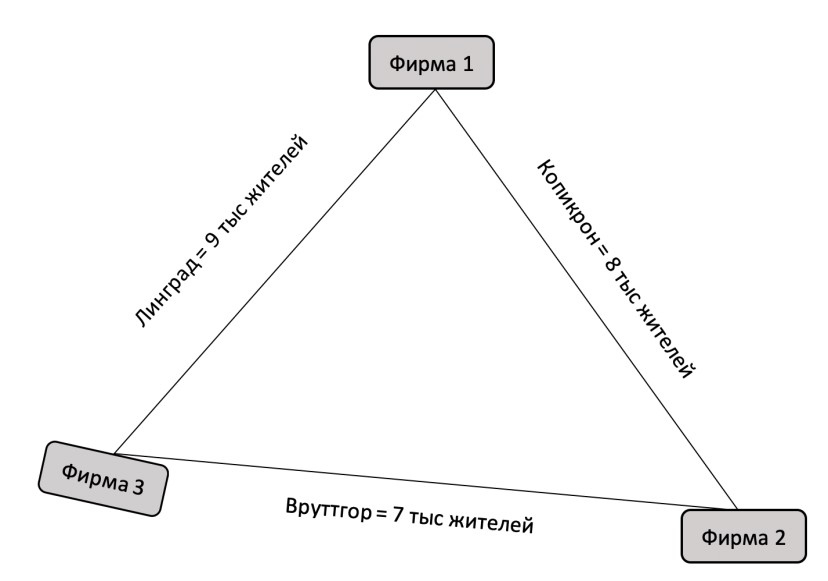
\includegraphics[width=0.5\linewidth]{static/4_9}
    \end{center}
    \indent\setlength{\parindent}{1em}\indent\setlength{\parindent}{1em}Известно, что в каждом городе жители
    распределены равномерно по всей его территории, и на каждый километр города приходится 1 тысяча жителей. На
    границах между городами расположены фирмы, производящие некоторое однородное благо.\\
    \indent\setlength{\parindent}{1em}Известно, что издержки первой фирмы на производство $q$ единиц блага составляют
    $aq$ денежных единиц ($a>0$), издержки второй фирмы – $bq$ денежных единиц ($b>0$), а издержки третьей фирмы – $cq$
    денежных единиц ($c>0$).\\
    \indent\setlength{\parindent}{1em}Каждый житель страны $N$ потребляет ровно одну единицу блага, которое он
    приобретает в одном из магазинов, расположенных на краю города (например, жители Копикрона никогда не покупают
    продукцию фирмы 3).\\
    \indent\setlength{\parindent}{1em}Удовольствие каждого жителя от потребления блага задается функцией:
    $$U(p,h)=15-p-h$$
    \indent\setlength{\parindent}{1em}где $p$ – цена блага, а $h$ – расстояние (в километрах) до фирмы, у которой житель
    приобрел благо.\\
    \indent\setlength{\parindent}{1em}Известно, что покупки в каждой фирме совершают жители из обоих городов, которым
    она доступна.\\
    \indent\setlength{\parindent}{1em}Найдите цены, которые установят фирмы.\bigskip\\
    \textit{\textbf{\centering\href{https://iloveeconomics.ru/sites/default/files/olimp/proba/2020/proba_2020_2020_ekonomika_2_etap_10_klass_19909.docx}{Решение}}}
\end{mybox}

\begin{mybox}{Задача 10. \textit{Всерос 2022}}
    \indent\setlength{\parindent}{1em}\indent\setlength{\parindent}{1em}Население деревни Вилларибо проживает равномерно
    на отрезке $[0; 1]$, а деревни Виллабаджо –– равномерно на отрезке $[2; 3]$. В Вилларибо и Виллабаджо приехал
    владелец сети магазинов «Кукумбрикс», который объявил, что сеть построит первый и единственный магазин в
    окрестности, а в какой точке прямой $(-\infty; +\infty)$ он будет построен –
    решать жителям деревень. Конечно, каждый житель хочет, чтобы магазин был построен как можно ближе к его дому.\\
    \indent\setlength{\parindent}{1em}Обычно все общие географические вопросы жители Вилларибо и Виллабаджо решают,
    используя механизм «Посередине между делегатами». А именно, сначала каждая деревня выбирает по одному делегату.
    Затем, если дом делегата Вилларибо находится в точке с координатой $a$, а дом делегата Виллабаджо имеет
    координату $b$, то решением вопроса является точка с координатами $\frac{a+b}{2}$. Делегатом $a$ будем называть
    того, который живет в точке с координатой $a$.\smallskip\\
    \indent\setlength{\parindent}{1em}\textbf{(a)} Изобразите на прямой $(-\infty; +\infty)$ множество всех точек, в
    которых хотя бы при какой-нибудь паре делегатов может быть построен магазин.\smallskip\\
    \indent\setlength{\parindent}{1em}\textbf{(b)} Докажите, что жителям Вилларибо для выбора делегата не нужна
    информация о делегате от Виллабаджо: если житель Вилларибо $x$ предпочитает делегата от Вилларибо $a_1$ делегату
    $a_2$ при делегате от Виллабаджо $b_1$, то житель Вилларибо $x$ предпочтет делегата от Вилларибо $a_1$ делегату $
    a_2$ при любом другом делегате от Виллабаджо $b_2$.\smallskip\\
    \indent\setlength{\parindent}{1em}\textbf{(c)} В этом и только в этом пункте считаем, что жители деревень выбирают
    в качестве делегата \textit{победителя по Кондорсе} – такого жителя деревни, что его предпочтет не менее половины
    жителей этой деревни при голосовании против любого другого жителя деревни (корректность определения следует из
    предыдущего пункта). Где будет построен магазин?\smallskip\\
    \indent\setlength{\parindent}{1em}\textbf{(d)} Говорят, что механизм принятия решений является манипулируемым,
    если существует такая пара делегатов от деревень, что хотя бы одному из делегатов выгодно скрыть настоящее место
    расположения своего дома и использовать для принятия решения какую-то другую координату. Докажите, что описанный
    механизм принятия решений является манипулируемым.\smallskip\\
    \indent\setlength{\parindent}{1em}\textbf{(e)} Предложите какой-нибудь механизм принятия решений, выдающий по паре
    делегатов $a$ и $b$ место для магазина и не являющийся манипулируемым.\bigskip\\
    \textit{\textbf{\centering\href{https://iloveeconomics.ru/sites/default/files/olimp/vseros/2022/vseros_2022_solutions_10_23379.pdf}{Решение}}}
\end{mybox}

\begin{mybox}{Задача 11. \textit{Всерос 2021}}
    \indent\setlength{\parindent}{1em}\indent\setlength{\parindent}{1em}Озеро Йутават представляет собой идеальный
    круг. Борис, Евгений и Максим ловят в этом озере рыбу и продают ее местным жителям, которые живут вокруг озера.
    Каждый день рыбаки независимо друг от друга выбирают, в каких точках на берегу (окружности) озера организовать
    продажу рыбы. Жители распределены вокруг озера равномерно (то есть на каждый километр расстояния вдоль окружности
    приходится одинаковое и достаточно большое число жителей). Цена килограмма рыбы исторически сложилась на
    определенном уровне, она достаточно высока, чтобы окупать усилия и снасти рыбаков, никто из них не считает
    уместным ее менять. Каждый рыбак ловит достаточно много рыбы, чтобы хватило любому количеству потребителей.\\
    \indent\setlength{\parindent}{1em}Каждый местный житель потребляет по 1 килограмму рыбы в день, покупая ее у
    ближайшего из трех рыбаков (по расстоянию, которое нужно проделать по окружности). Если расстояние от потребителя
    до двух ближайших рыбаков одинаково, то он принимает решение произвольным образом (этим потребителем можно
    пренебречь). Рыбаки, таким образом, конкурируют за потребителей, и каждый из них хочет выбрать своё расположение
    на берегу озера так, чтобы максимизировать выручку. Два или три рыбака могут выбрать одну и ту же точку для
    продажи, в таком случае они будут делить выручку на равные части.
    \begin{center}
        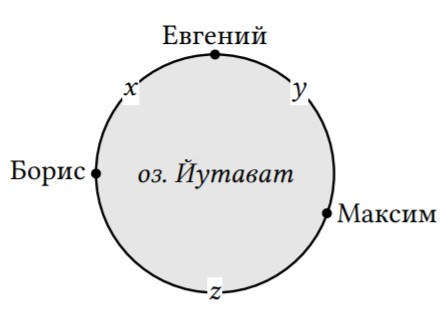
\includegraphics[width=0.5\linewidth]{static/4_11}
    \end{center}
    \indent\setlength{\parindent}{1em}\indent\setlength{\parindent}{1em}По итогам каждого дня каждый рыбак оценивает
    объем продаж за день и следующим образом принимает решение, где организовать продажи на следующий день:
    \begin{enumerate}
        \item Если его сегодняшнее положение принесло ему максимальную дневную выручку среди всех вариантов его
        размещения (с учетом фактического положения двух других), то на следующий день он остается в той же точке.
        \item Если условие предыдущего пункта не выполнено, он выбирает какую-то другую точку, в которой при текущем
        расположении других рыбаков его выручка была бы больше.
    \end{enumerate}
    \indent\setlength{\parindent}{1em}По прошествии нескольких дней все рыбаки решили больше никуда не двигаться и
    навсегда остались в некоторых точках (такое расположение является равновесием Нэша в этой задаче). Опишите их все
    возможные финальные расположения через ограничения на параметры $x,y,z$ (расстояния между рыбаками). Считайте, что
    длина окружности $x+y+z=1$\bigskip\\
    \textit{\textbf{\centering\href{https://iloveeconomics.ru/sites/default/files/olimp/vseros/2021/vseros_2021_solutions_10_21648.pdf}{Решение}}}
\end{mybox}

\begin{mybox}{Задача 12. \textit{Всерос 2018}}
    \indent\setlength{\parindent}{1em}\indent\setlength{\parindent}{1em}В стране A есть четыре города и прямые дороги
    между ними. Расположение городов и дорог, а также расстояния между городами изображены на картинке. В скобках
    указано население городов в миллионах человек.
    \begin{center}
        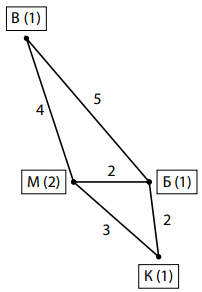
\includegraphics[width=0.5\linewidth]{static/4_12}
    \end{center}
    \indent\setlength{\parindent}{1em}\indent\setlength{\parindent}{1em}Государство думает, где именно расположить
    мусорную свалку. Для возможности транспортировки мусора свалка может находиться только непосредственно на обочине
    дороги или в самих городах. Конечно, жители каждого города хотят, чтобы свалка была как можно дальше от их города
    (для простоты будем считать, что они имеют в виду расстояние, которое нужно проехать по дороге).\smallskip\\
    \indent\setlength{\parindent}{1em}\textbf{(a)} Назовем точку X доминирующим местом для свалки, если она победила
    бы во всеобщем голосовании жителей страны, будучи выставленной против любой другой точки, по правилу простого
    большинства голосов. При правиле простого большинства побеждает тот вариант расположения, который получает строго
    больше половины голосов всех жителей. При безразличии жителей города между двумя вариантами считайте, что они
    разделяют свои голоса поровну между предлагаемыми вариантами.\smallskip\\
    \indent\setlength{\parindent}{1em}Есть ли в стране A доминирующее место для свалки? Если есть, найдите его; иначе
    докажите, что его нет.\smallskip\\
    \indent\setlength{\parindent}{1em}\textbf{(b)} Назовем точку Y неудачным местом для свалки, если существует такая
    точка Z, что жители по меньшей мере трех городов строго предпочитают точку Z точке Y. Найдите множество неудачных
    мест для свалки.\smallskip\\
    \indent\setlength{\parindent}{1em}\textbf{(d)} Глава государства Джон Ролз решил разместить свалку таким образом
    , чтобы ни один город не был особенно ущемлен: решение принимается так, чтобы свалка была как можно дальше от
    ближайшего к ней города. Где будет размещена свалка?\bigskip\\
    \textit{\textbf{\centering\href{https://iloveeconomics.ru/sites/default/files/olimp/vseros/2018/vseros_2018_vseros_10-11_klass_1_tur_resheniya_18405.pdf}{Решение}}}
\end{mybox}

\end{document}